\chapter{State of the art}\label{sec:Estado_arte}
In the following section, theoretical aspects will be considered for a correct understanding of the work done. In addition, the evolution of some systems will be presented, as well as its advantages and disadvantages.
\section{FPGA concept}
An FPGA\cite{FPGAWhat} (Field Programmable Gate Arrays) is a reconfigurable device that can be electrically programmed to implement a high variety of logic circuits. It consists in a uniform logic programmable structures array which are interconnected by configurable routing network. A routing network example is shown in \ref{fig:estructura_FPGA}.

\begin{center}
	\begin{figure}[H]
		\center
		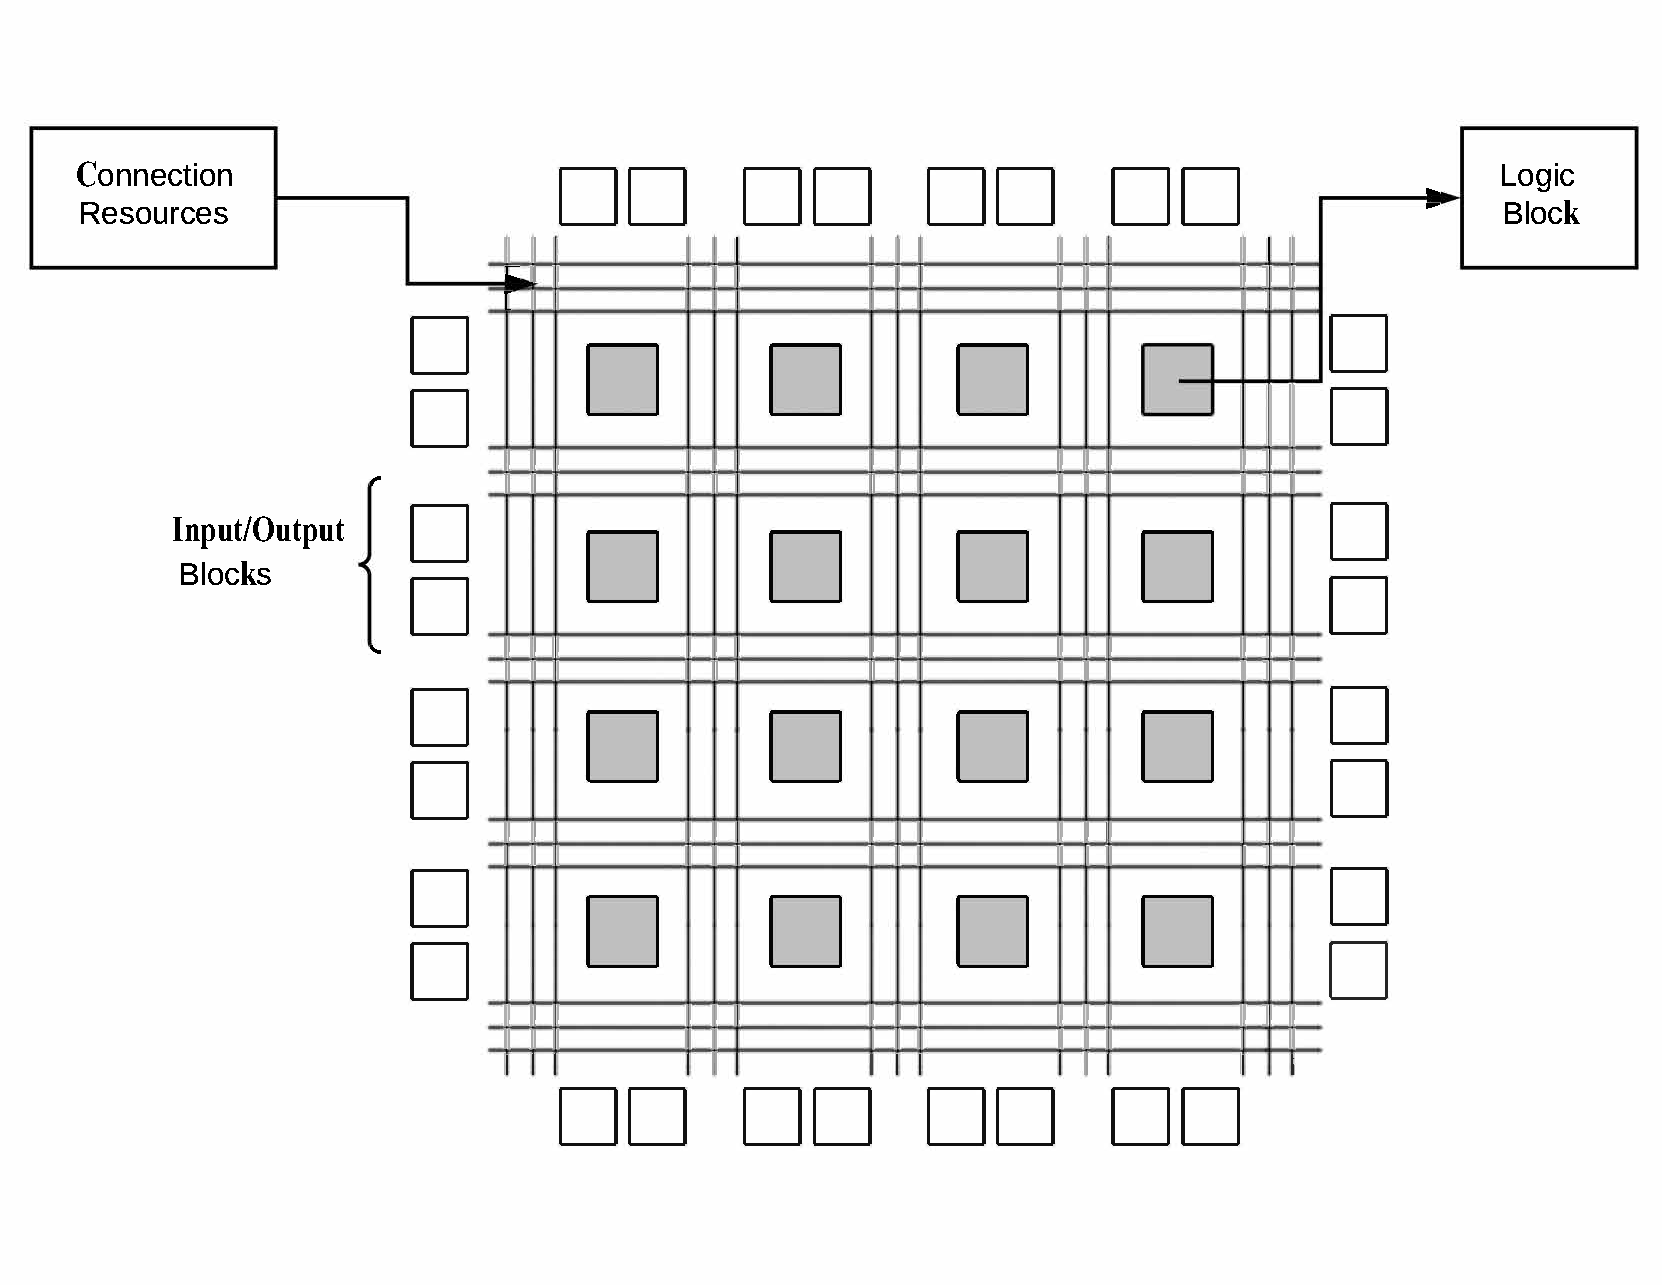
\includegraphics[trim = 0mm 10mm 0mm 10mm, clip,scale=0.4]{imagenes/EstadoArte/estructura_FPGA.pdf}
		\caption{PLD vs FPGA}
		\label{fig:estructura_FPGA}
	\end{figure}
\end{center}

The logic and structures interconnection can be configured thanks to the powerful CAD tools, which allow that the final user could define this physical logic blocks interconnection through Hardware Description Language (HDL). Some of the best known are the VHDL or ABEL. Although it is not the most used nowadays, along the \ref{sec:Verilog} section a brief introduction to Verilog will be done, discussing and analyzing its main features.
\subsection{Evolution and scenario}

FPGAs were invented in 1984 by Ross Freeman and Bernard Vonderschmitt, co-founders of Xilinx\cite{Xilinkx}. They were mainly designed to work as prototypes or demonstrations of digital electronic circuits. FPGAs conform the maximum evolution of PLDs (Programmable Logic Device), defined as integrated circuits which can be programmed Boolean Logic equations. Some usage examples nowadays are:
\begin{itemize}
	\item Artificial Vision Systems
	\item Medical Image Systems
	\item Coding and Encryption
	\item Voice Recognition
	\item Aeronautics and Defense
\end{itemize}

Revolutionary success from this programmable device can be attributed to the flexibility in design implementation. This way, the capacity to instantly reprogram the FPGA with several circuits without additional cost, promotes the reuse of the device and allows a fast design verification y because of that, reduces the cost in the developing stage. Even though they do not actually represent the whole system from a final product, its advantages in the properties of the design are making them to become much more important in the electronic products developing. \newline

In order to try to understand the importance of hardware implementation devices, it would be adequate to introduce the Moore’s Law. Moore’s Law expresses that approximately every 22 years, the number of transistors is duplicated in a
microprocessor. As it is shown in \ref{fig:Ley_de_Moore}, this law formulated by the Intel cofounder, E. Moore, in April the 19th of 1965, is not so far from reality.
\newline
\begin{figure}[H]
	\center
	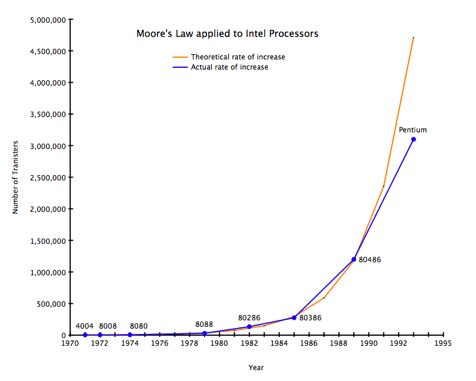
\includegraphics[scale=0.7]{imagenes/EstadoArte/MooresLaw.png}
	\caption{Moore's Law}
	\label{fig:Ley_de_Moore}
\end{figure}
 

However, as it has been announced form the main microprocessors enterprises like Intel and AMD, in their technological roadmap for semiconductors, the Moore’s Law will get to its end in 2021. After this date, it won’t be economically efficient to keep reducing the silicon transistor’s size. The industry prediction is not only that its reduction rate will become slower and slower, but that will definitely stop. At that point, digital electronics will start to have an important role with microprocessors. This is forcing Multinational Enterprises dedicated to Microprocessors manufacturing like Intel or AMD, to implement those behaviors in FPGAs. Its advantages and disadvantages will be presented in \ref{sec:ArquitecturaFPGA} and \ref{sec:DescripcionHardware}.
\newpage
\subsection{FPGA Architecture}\label{sec:ArquitecturaFPGA}

In a PLD, interconnections between elements is already prefixed and it is only possible to enable or disable this connection. Otherwise, FPGAs connections are no prefixed, making possible to the final user to decide the logic blocks interconnections. (figura \ref{fig:pld_fpga}).
\newline
\begin{center}
\begin{figure}[H]
	\center
	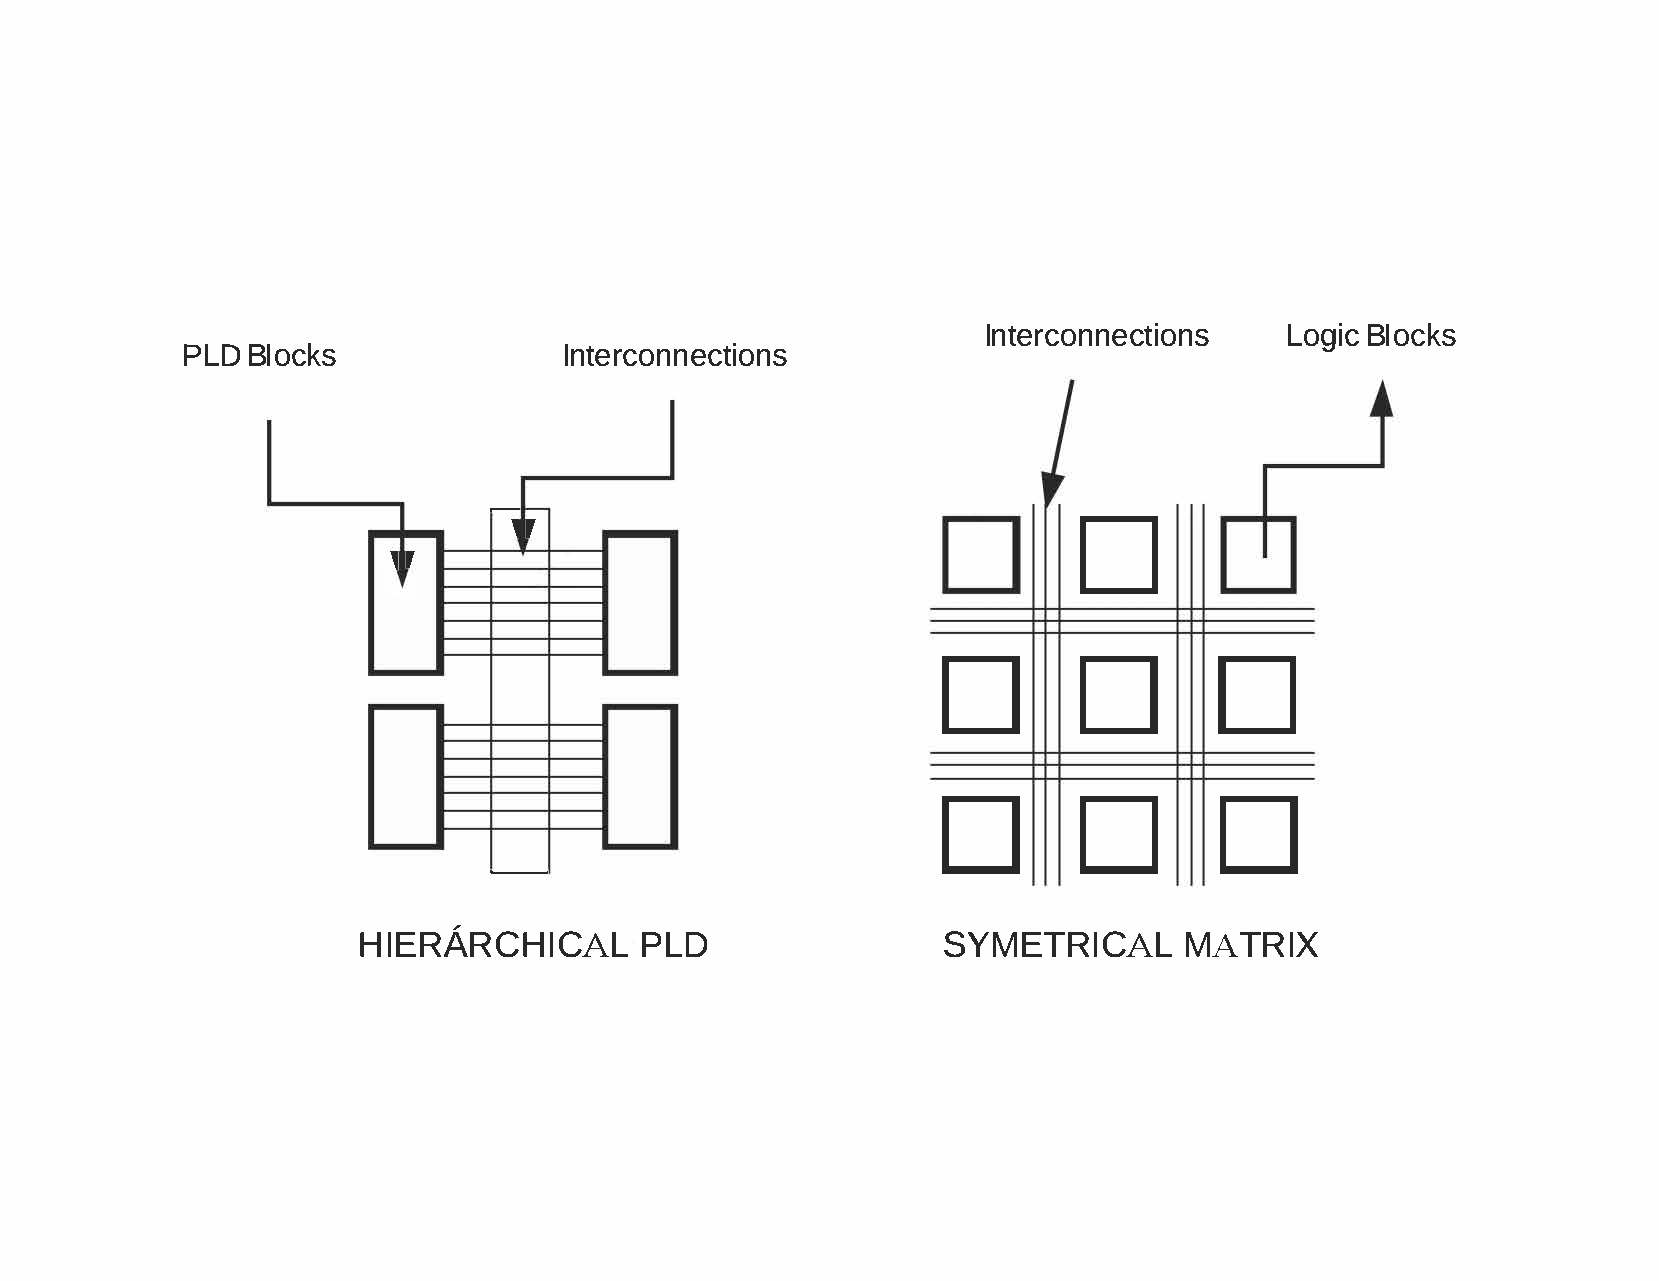
\includegraphics[trim = 10mm 35mm 10mm 35mm, clip,scale=0.4]{imagenes/EstadoArte/pld_fpga.pdf}
	\caption{PLD vs FPGA}
	\label{fig:pld_fpga}
\end{figure}

\end{center}

When choosing a FPGA for a specific project, it is important to keep in mind one of its most important property: The number of logic blocks. This number determines the device capability and is part of one the most limited features from nowadays FPGAs/ Logic blocks are independent between them and are able to interconnect in order to build a more complex module. \newline

Now fine-grained and coarse-grained meanings will be introduced, which will lead to the correct understanding to the FPGA architecture. 

This complex module performs the basic operation which together represent the function that will operate in a FPGA. It is said that FPGAs are Advanced Architecture devices because of the density of its components and because of the different interconnection paths between modules. According to the module types that conform it, we have two structural configurations:
\begin{itemize}
	\item Fine-grained
	\item Coarse-grained
\end{itemize}

Logic modules in a coarse-grained architecture are big modules generally consistent which have one or more query tables and two or more Flip-Flops. The query table is also known as the Look Up Table (LUT). It performs like a memory where the truth table, which represents the circuit logic function is located, this way, any desired function could be implemented in a LUT. Depending of the LUT size, more or less variable functions can be implemented.\newline

On the other hand, a fine-grained architecture is structured by a huge quantity of small logic modules which perform relatively simple tasks. Each module has a two-input circuit that performs a determined logic function, or in some other cases by a multiplexor. It may also contain any Flip-Flop. \newline

The most used FPGAs nowadays have the coarse-grained technology, which allows to increase the abstraction level with respect to fine-grained FPGAs. \newline

The first case allows less detailed implementations since from a very low level there are much more complex modules and the fact of using LUT suggests that larger designs can be created. Along this project the first case will be considered, as an example of that is the FPGAs used, IceZum Alhambra II.\newline

The designer proposes the logic function to be performed throughout the description hardware methods and define the parameter to its design. This is done through programmable code, that can be a description hardware language, which is introduced in section \ref{sec:DescripcionHardware}. 

\subsection{Hardware Description Languages}\label{sec:DescripcionHardware}

A Hardware Description Language\cite{HDL} (HDL) is a language used to model the hardware block functionality in a textual way. As we can find differences between the different type of programming languages according to their coding syntax and their simulation methods and synthesis, we can find several differences between HDLs. There are two different hardware description languages types:
\begin{itemize}
	\item Low level: They do not allow the hierarchy of modules and they are able to perform only simple descriptions.
	\item High level: They are the most used currently, they allow to design more complex systems. Examples of high modeling are Verilog (Verify Logic) and VHDL (VHSIC Hardware Description Language).
\end{itemize}	
This work would be based on Verilog for allowing a higher level of implementation than VHDL, as would be discussed in section \ref{sec:Verilog}. \newline

Both languages share some common characteristics, such as support for any level of modeling and abstraction, and that each design element has well defined interphase to allow fast connection with other logical elements.

\subsection{Verilog}\label{sec:Verilog}
Due to its use throughout this project, some important characteristics, whose knowledge would be basic to understand the code, will be analyzed.

\subsubsection{Type of data}

There are two types of data in Verilog which must be understood in order to reach the desired functionality:
\begin{itemize}
	\item reg: Represent variables with information storage capacity.
	\item wire: They represent connections between components, they do not have storage capacity.
\end{itemize}

\subsubsection{Modules Implementation}
In most cases and in order not to lose the abstraction level, a project in Verilog\cite{496013} is usually composed of a set of modules which form a complete functionality, and each of them, a specific one. \newline

The main features of the digital implementation by modules are:
\begin{itemize}
	\item Each module has a series of inputs and outputs whose main function is to interconnect other modules, although it may not have inputs and outputs.
	\item Each module can be described architecturally or behavioral.
\end{itemize}

This implementation by Verilog modules allows the configuration of the abstraction level desired by the end user. The development of specific functionality modules can have their advantages and disadvantages depending on their final use. If they want to be reused for other workflows (example: 8-bits adder), it is good to have very defined modules according to their functionality (example: 2-bit adder). However, polarization does not have to be essential, although advised.

\subsubsection{Process Parallelism}
One of the most important features that differentiates Verilog from the rest of the procedural languages \footnote{Procedural Languages: The application execution starts in the code’s first line and follows a predefined root through the application, calling procedures as it is necessary.} is the possibility of executing several processes in parallel, a fundamental aspect in the language which provides a great part of the advantages of using hardware implementation.

\begin{center}
	\begin{figure}[H]
		\center
		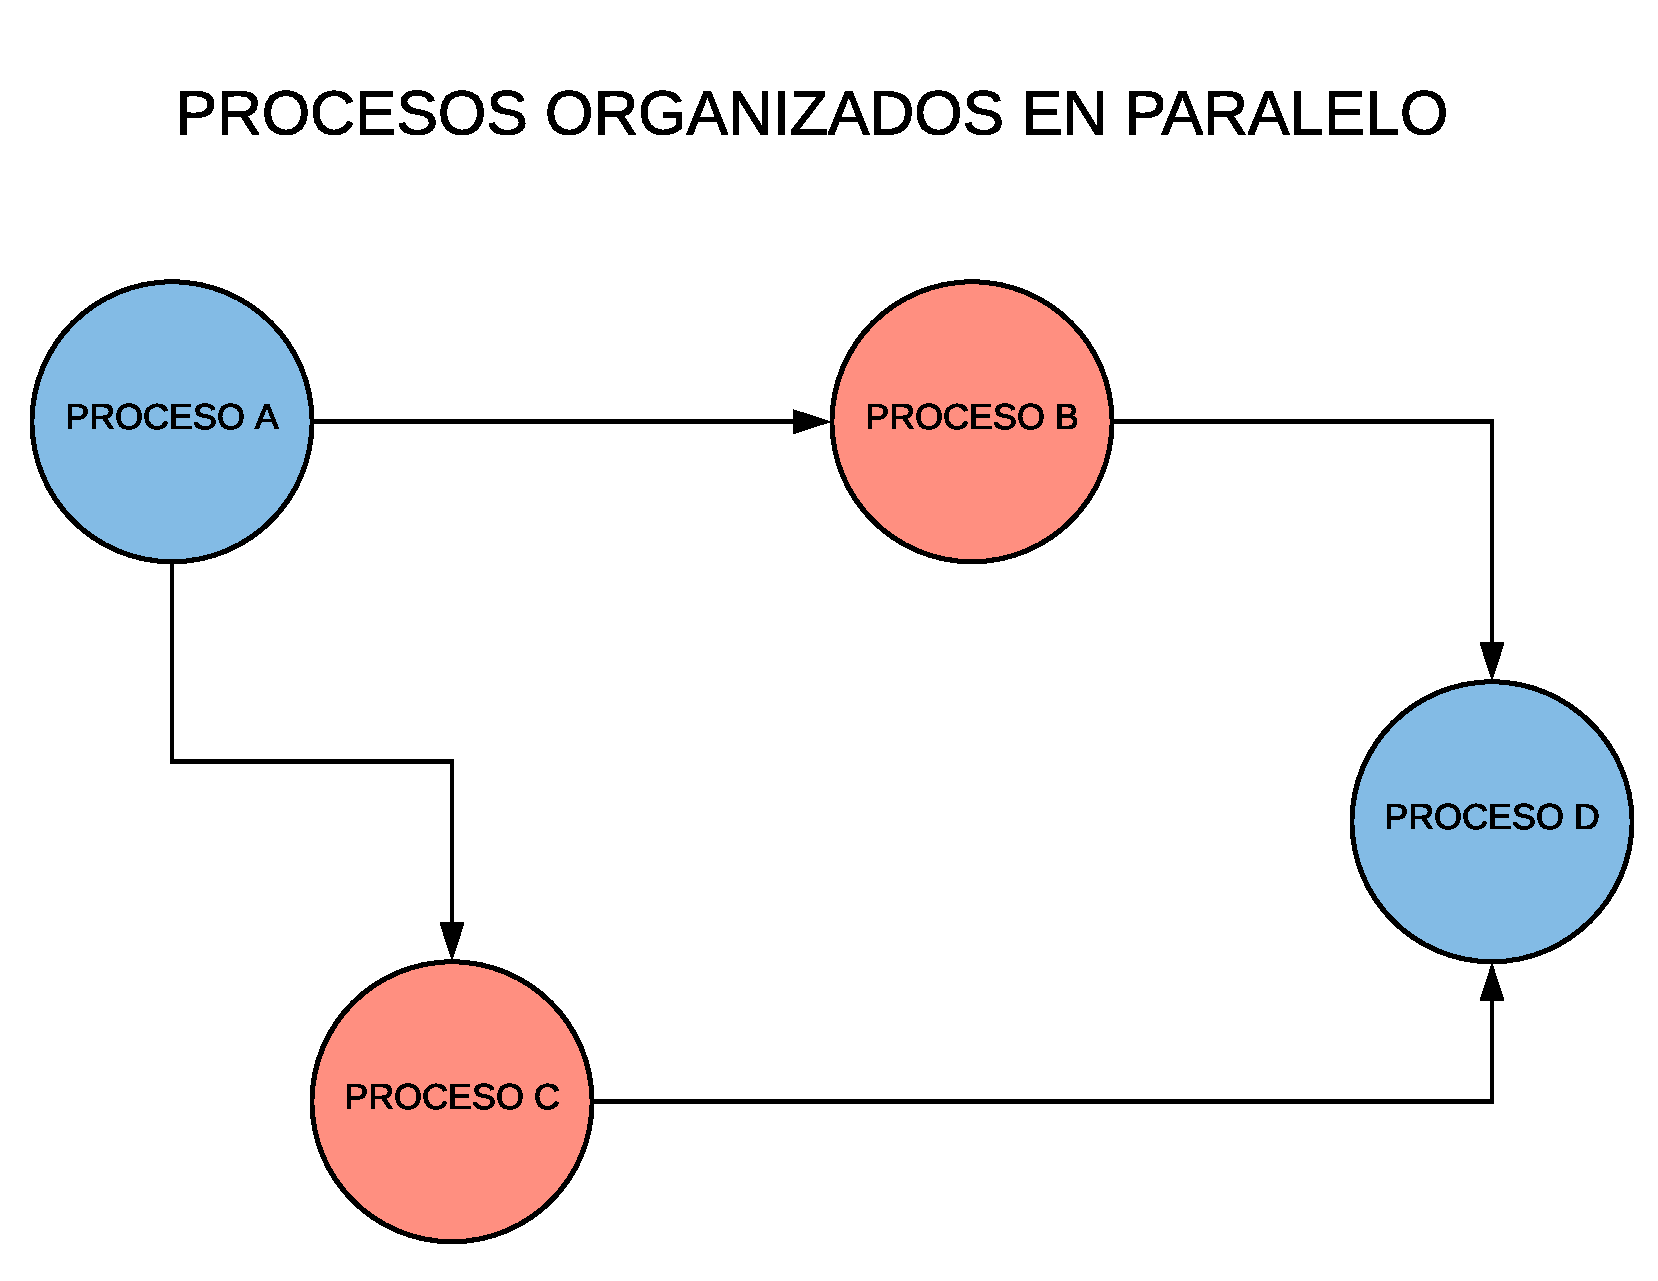
\includegraphics[trim = 0mm 0mm 0mm 0mm, clip,scale=0.3]{imagenes/EstadoArte/procesos_paralelo.pdf}
		\caption{Process Parallelism}
		\label{fig:procesos_paralelo}
	\end{figure}
	
\end{center}
The whole implementation of Verilog is declared inside a process that can be of two types:
\begin{itemize}
		\item Initial: This type of process is executed only once starting its execution at the beginning, therefore, there are no delays. This process is not synthesizable, which means it cannot be used in an RTL description.
		
		\item Always: This type of process is continuously executed as a loop, as its own name indicates, is continually running. This is a synthesizable process and is controlled by timing or events. If this block is executed by more than one event, its set is called sensitive list.
\end{itemize}

\subsubsection{Control Structures}

Just like other procedure languages, Verilog has a series of control structures:

\begin{itemize}
	\item if - else
	\item Case. This is one of the most used along this project. It allows the state machines generation.
	\item For
	\item While
	\item Forever
	\item Wait
	
\end{itemize}

\subsubsection{Continuous Assignment}

Through continuous assignment a logic combinational can be modeled, that means, there’s no need a sensibility list to complete the task. It can only be declared outside of any process.

\subsubsection{Procedural Assigment}

Variables have a value assigned inside an always or initial process, the type of variable to which the value is assigned can be of any type.
%%%%%%%%%%%%%%%%%%%%%%%%%%%%%%%%%%%%%%%%%%%%%%%%%%
\newpage
\section{Open FPGAs evolution}
Many hardware implementation languages as well as its FPGA architecture used, are linked to important companies such as Xilinx, Intel (formerly Altera), etc, and being able to work with them requires a large budget. \newline
This leads us to the fact that not many companies or individuals can benefit from the advantages of using FPGAs, and at the same time, that technological progress is at a slower rate. One of the keys of success of companies like Arduino is not more than the community of people that stands behind creating new libraries, components, etc. This is all thanks to the low price of its products and the possibility of finding all the hardware and software on the web. \newline

To understand the formation of free FPGAs it is important to know what the bytestream is. \newline
A bytestream is a sequence of bytes that is used in telecommunications and IT. The term bytestream is used to describe the configuration with which a specific design will be implemented in an FPGA. This detailed bitstream format for a particular FPGA is typically owned by the FPGA provider. \newline

This is why Clifford Wolf decided to interpret the bytestream of the Lattice\cite{Lattice} iCE40 model and developed the IceStorm\cite{7910719} tool. \newline
IceStorm was developed as a translate software from Verilog (Description Language in FPGAs, \ref{sec:Verilog}) and bytestream. This translation was possible thanks to the inverse engineering, this means that the usual usage is not give, but the inverse.

There’s no longer dependency on any manufacturer and all knowledge is also available. From these tools you can create any interface or any application that has not been foreseen by the manufacturer. \newline

Only Lattice iCE40 FPGAs (HX1K-TQ144 and HX8K-CT256 models) are at the moment the ones that can be worked with (figura \ref{fig:lattice}), but since it is a open project \footnote{Open project: This refers to the user freedom to execute, copy, distribute, study, change and improve that hardware or software.},a lot of people are increasing their chances.
\begin{center}
	\begin{figure}[H]
		\center
		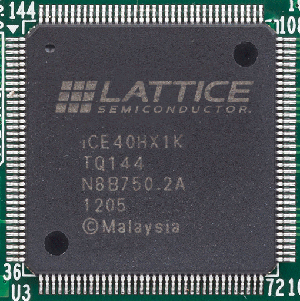
\includegraphics[trim = 0mm 0mm 0mm 0mm, clip,scale=0.4]{imagenes/EstadoArte/lattice.png}
		\caption{Lattice iCE40HX1K}
		\label{fig:lattice}
	\end{figure}
\end{center}
\newpage
Some FPGAs examples that are now available for users are shown in figures \ref{fig:tiny_fpga}, \ref{fig:blackIceII}, \ref{fig:icoBoard}
\begin{center}
	\begin{figure}[H]
		\center
		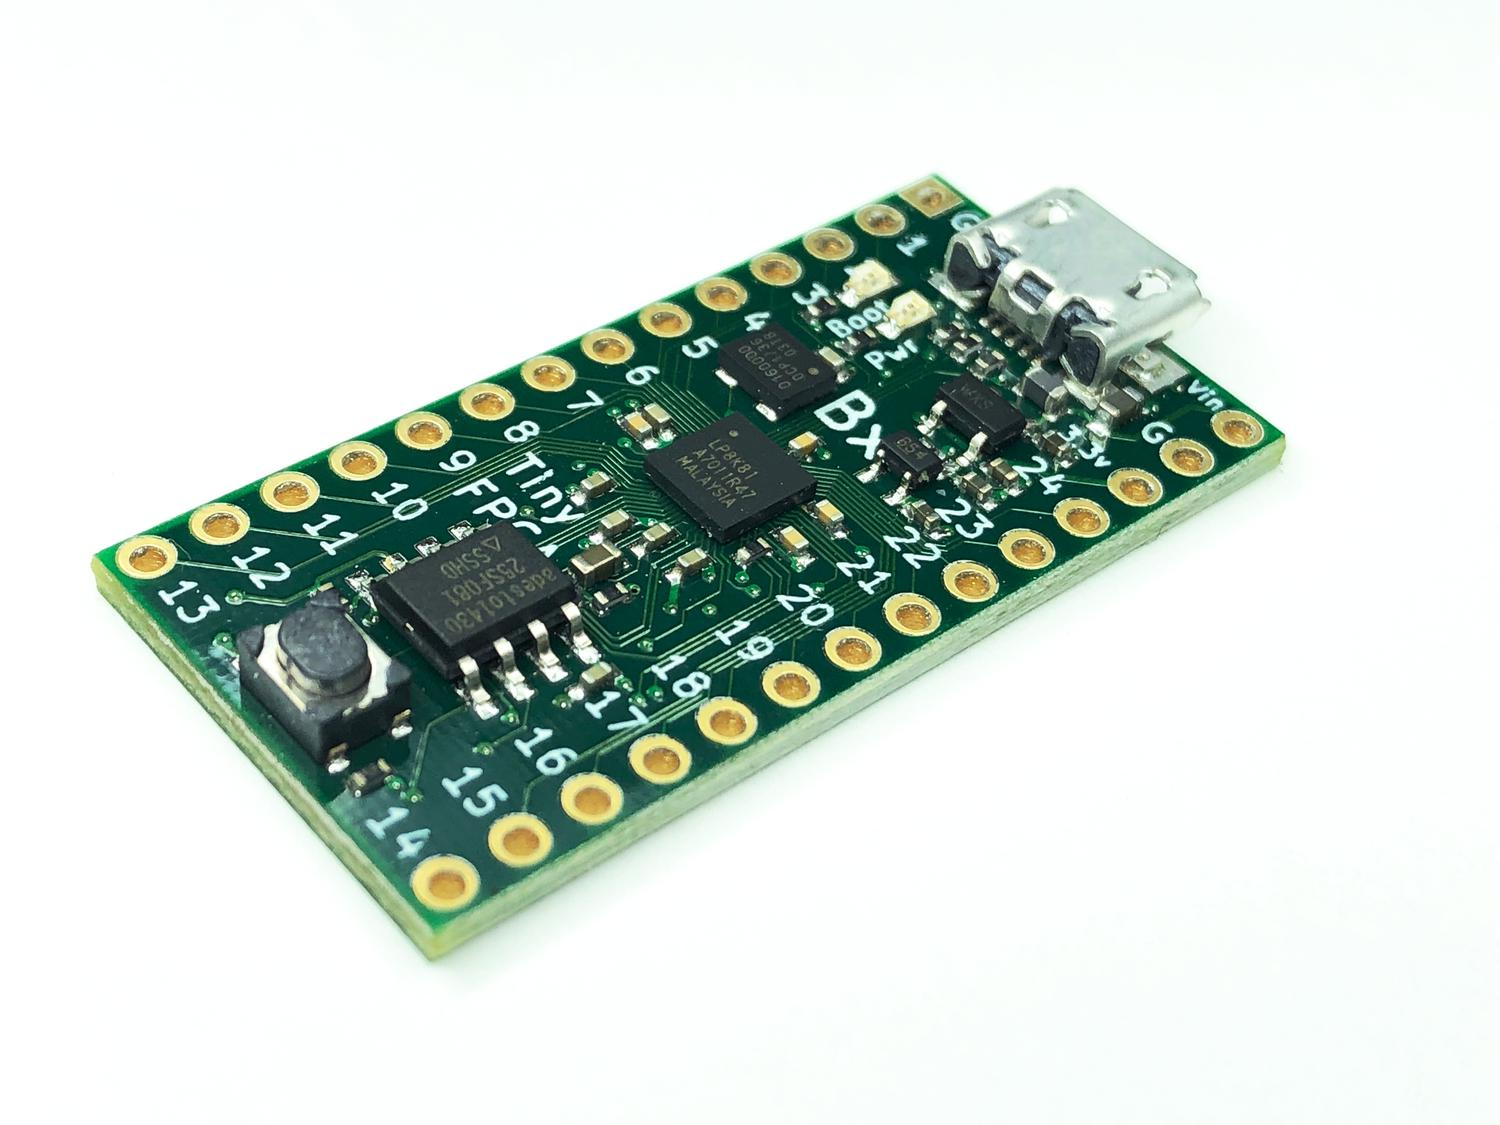
\includegraphics[trim = 0mm 0mm 0mm 0mm, clip,scale=0.15]{imagenes/EstadoArte/tinyFPGABX.jpg}
		\caption{Tiny FPGA BX}
		\label{fig:tiny_fpga}
	\end{figure}
\end{center}
\begin{center}
	\begin{figure}[H]
		\center
		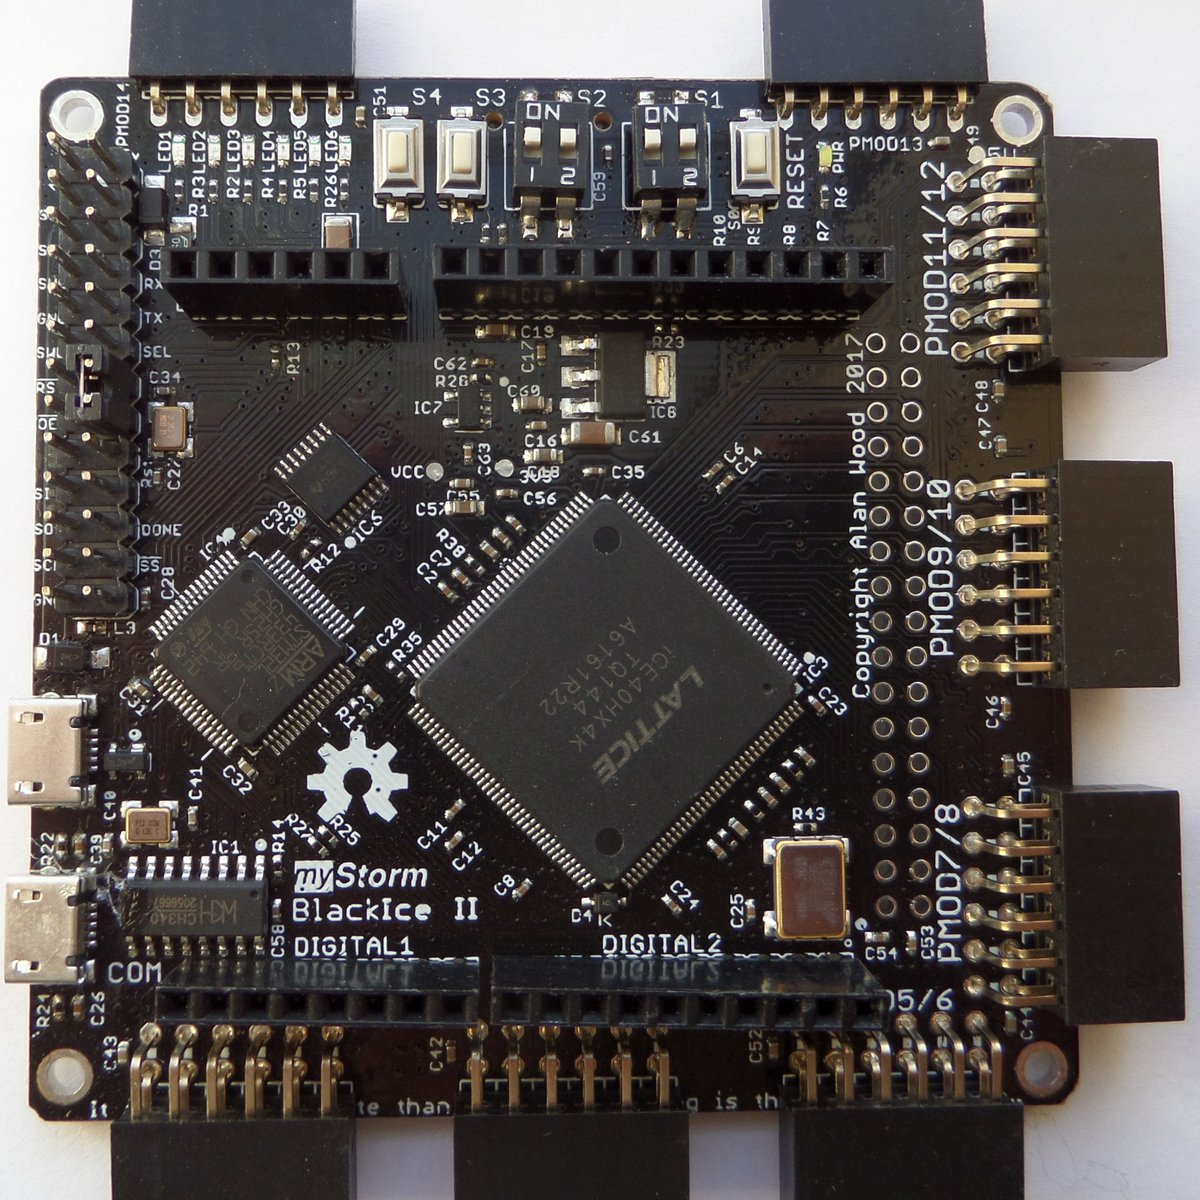
\includegraphics[trim = 0mm 0mm 0mm 0mm, clip,scale=0.1]{imagenes/EstadoArte/BlackIce.jpg}
		\caption{BlackIce II}
		\label{fig:blackIceII}
	\end{figure}
\end{center}
\begin{center}
	\begin{figure}[H]
		\center
		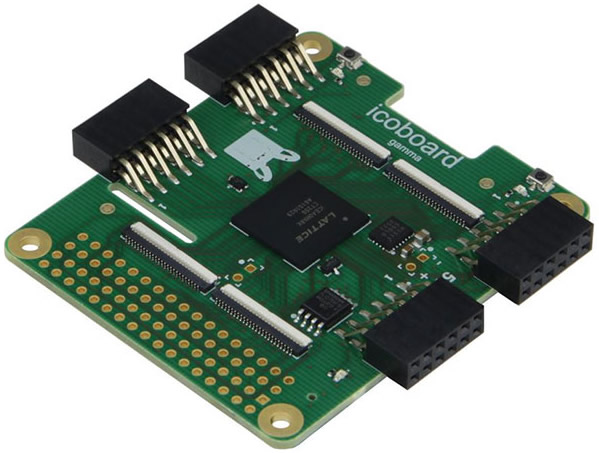
\includegraphics[trim = 0mm 0mm 0mm 0mm, clip,scale=0.3]{imagenes/EstadoArte/ico_board.jpg}
		\caption{ico Board}
		\label{fig:icoBoard}
	\end{figure}
\end{center}
\subsection{IceZum Alhambra}
For this project, IceZum Alhambra\cite{Alhambra} has been used, which has been completely designed and assembled in Granada (Spain).\newline
This is a free FPGA compatible with IceStudio (to be analyzed in section \ref{sec:IceStudio}). Some of its most important features are:
\begin{itemize}
	\item Development FPGA board iCE40HX1K-TQ144 from Lattice company. 
	\item Open hardware.
	\item Compatible with IceStorm toolchain.
	\item Compatible with Arduino Uno shields. 
	\item 12MHz oscillator.
	\item ON/OFF switch to enable or disable digital pins.
	\item 20 Input/Output 5V pins.
	\item 8 Input/Output 3.3V pins.
	\item Micro-B USB to program FPGA from PC.
	\item Reset button.
	\item 8 general purpose LEDs.
	\item TX/RX LEDs.
	\item 4 analogic inputs available through i2c.
\end{itemize}

It is known that there are better features board, but the fact that it is Open Hardware and that can be implemented with IceStudio, has led to the final choice of this board for the development of this project.\newline
\begin{center}
\begin{figure}[H]
	\center
	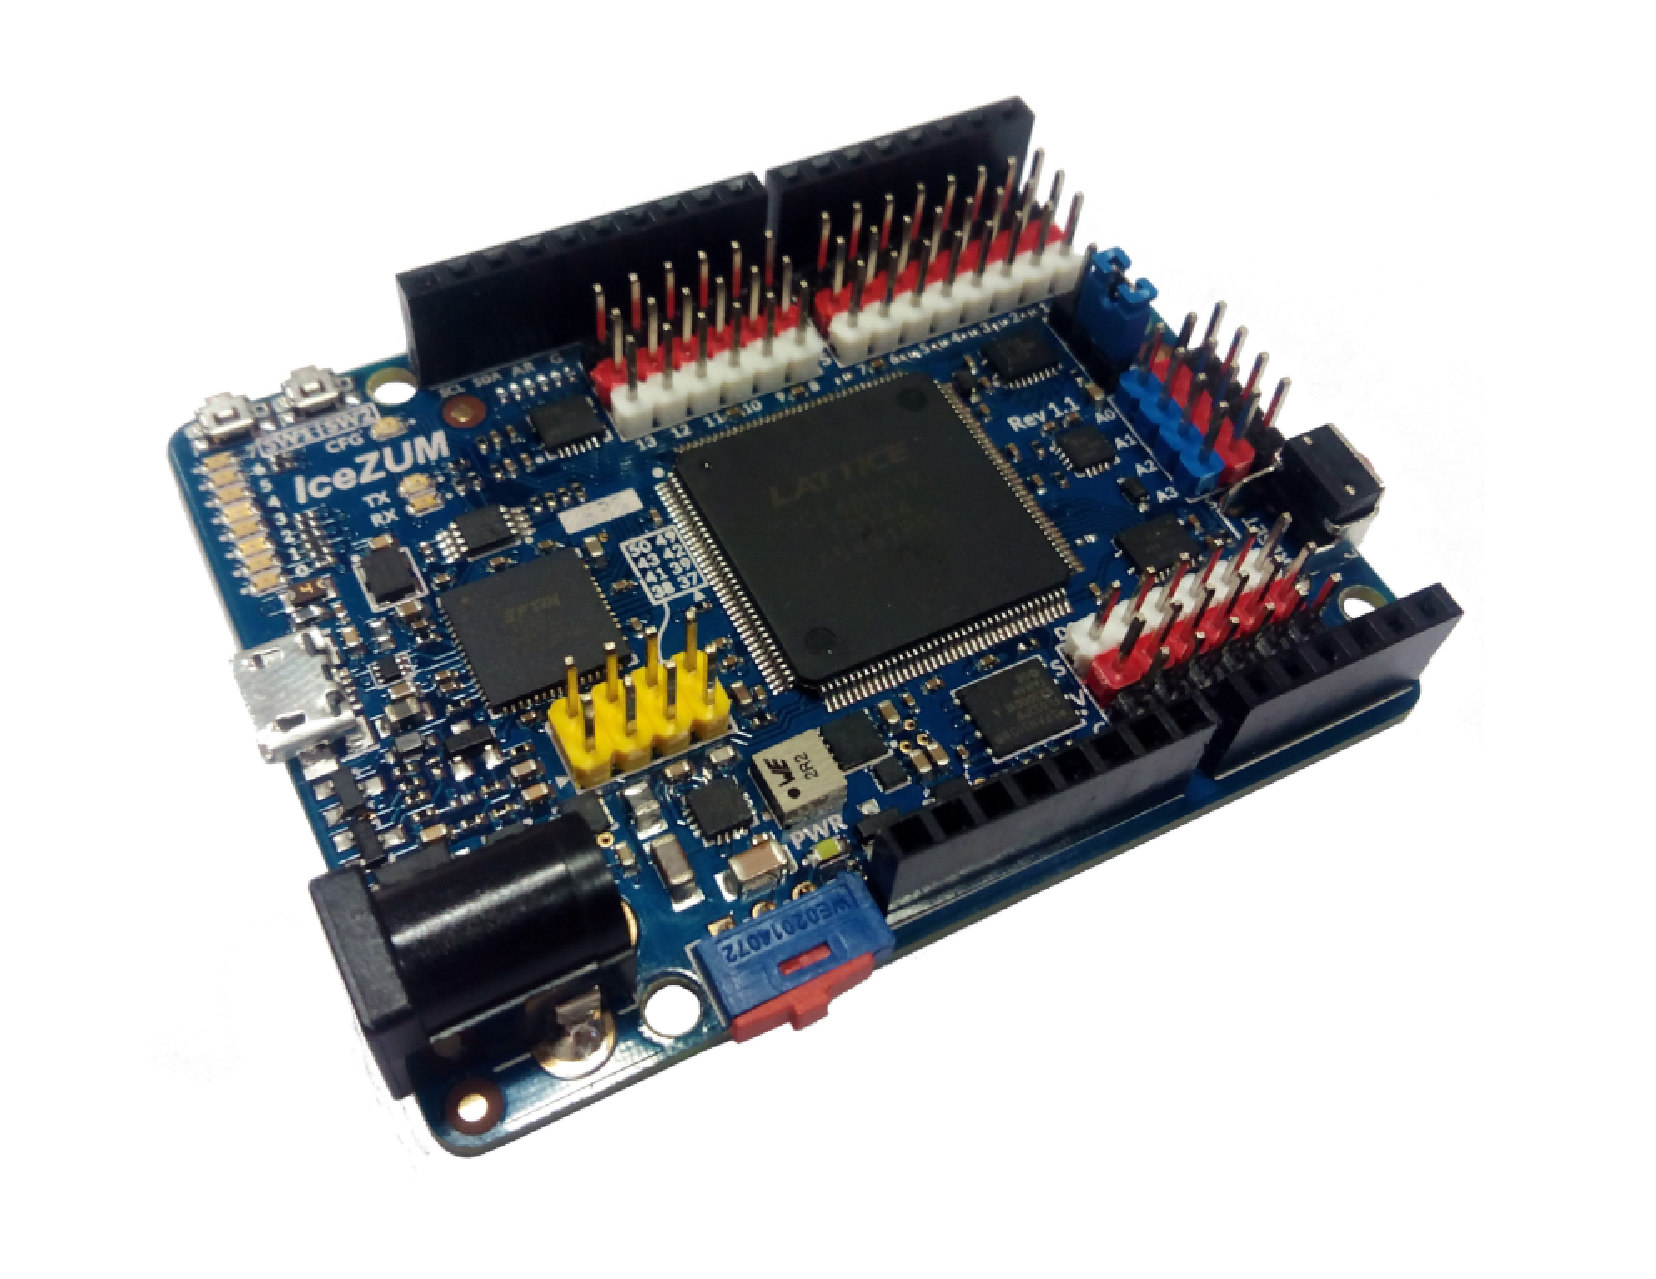
\includegraphics[scale=0.4]{imagenes/EstadoArte/IceZumAlhambra.pdf}
	\caption{IceZum Alhambra Board}
	\label{fig:IceZumAlhambraI}
\end{figure} 
\end{center}
One point to keep in mind for the hardware development with this FPGA is its 1K memory, which has been a significant limitation in the development. For the present project, the new version of the IceZum Alhambra, IceZum Alhambra II, was also used, which was not in the market at the beginning of the project and which takes some improvements, such as the expansion of 8K in its memory, the improvement of the data bus i2c, the possibility of powering through LIPO. battery, etc. IceZum is presented in figure \ref{fig: IceZumAlhambraII}.
\begin{center}
	\begin{figure}[H]
		\center
		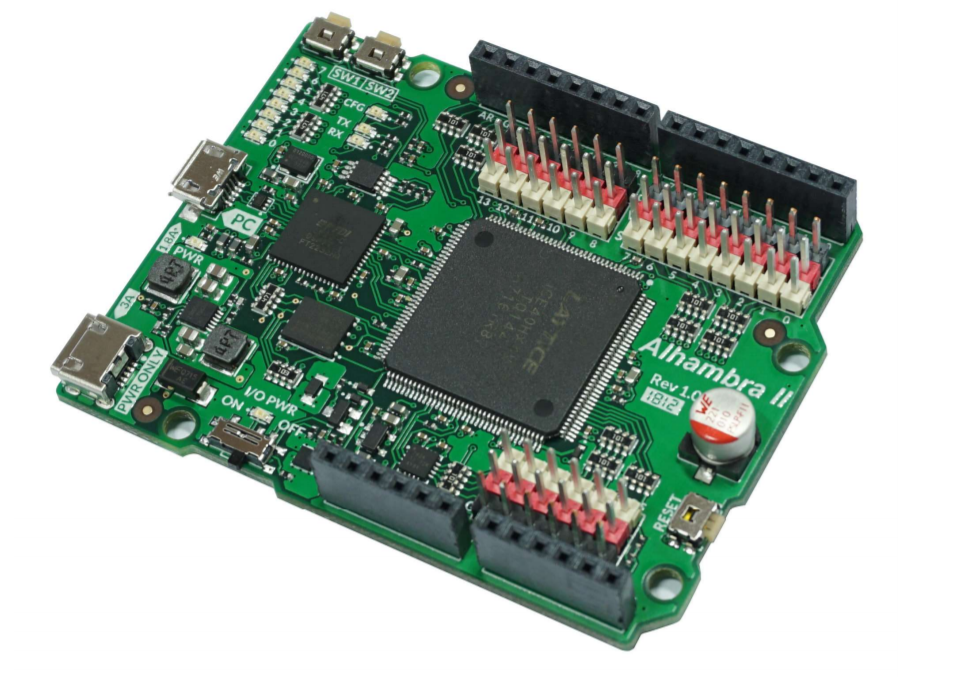
\includegraphics[scale=0.5]{imagenes/EstadoArte/IceZumAlhambra.PNG}
		\caption{IceZum Alhambra II Board}
		\label{fig: IceZumAlhambraII}
	\end{figure} 
\end{center}


\subsection{IceStudio}\label{sec:IceStudio}
HDL languages usually have a difficult learning curve, this is largely due to the low level of abstraction needed to design a particular system. It is necessary to know the hardware features of our system in order to work with this type of logic. \newline

As previously developed, some manufacturers provide commercial tools to program their own FPGAs. Although in the present, they are complex environments, they have a great number of tools and functionalities. Unfortunately, most of them are not free and are linked to the architecture of a unique manufacturer.
\newline
With the evolution of FPGAs, languages that allow a higher level of abstraction have started to appear. In addition, tools focused on the implementation of graphic design have also appeared. An example of this type of implementation is LabVIEW FPGA or IceStudio\cite{IceStudio}. \newline
IceStudio is an Open Source project developed by Jesús Arroyo Torrens, on which the present document will be based. \newline

IceStudio is a graphic IDE for free FPGAs and is built on the IceStorm project. The objective of the IceStorm project is the reverse engineering and the bitstream format of the FPGA Lattice iCE40 (although a few more were emerging) documentation. It provides simple tools to analyze and create bitstream files, that is, the lowest level of implementation for an FPGA.\newline

To get the reader closer to the knowledge and operation of IceStudio, a series of representative screenshots will be incorporated throughout the document so that the vision of what is being done is not lost. For example, the main window of IceStudio and on which everything else will be developed, is the same as shown in figure \ref{fig:Main_IceStudio}. \newline

\begin{figure}[H]
	\center
	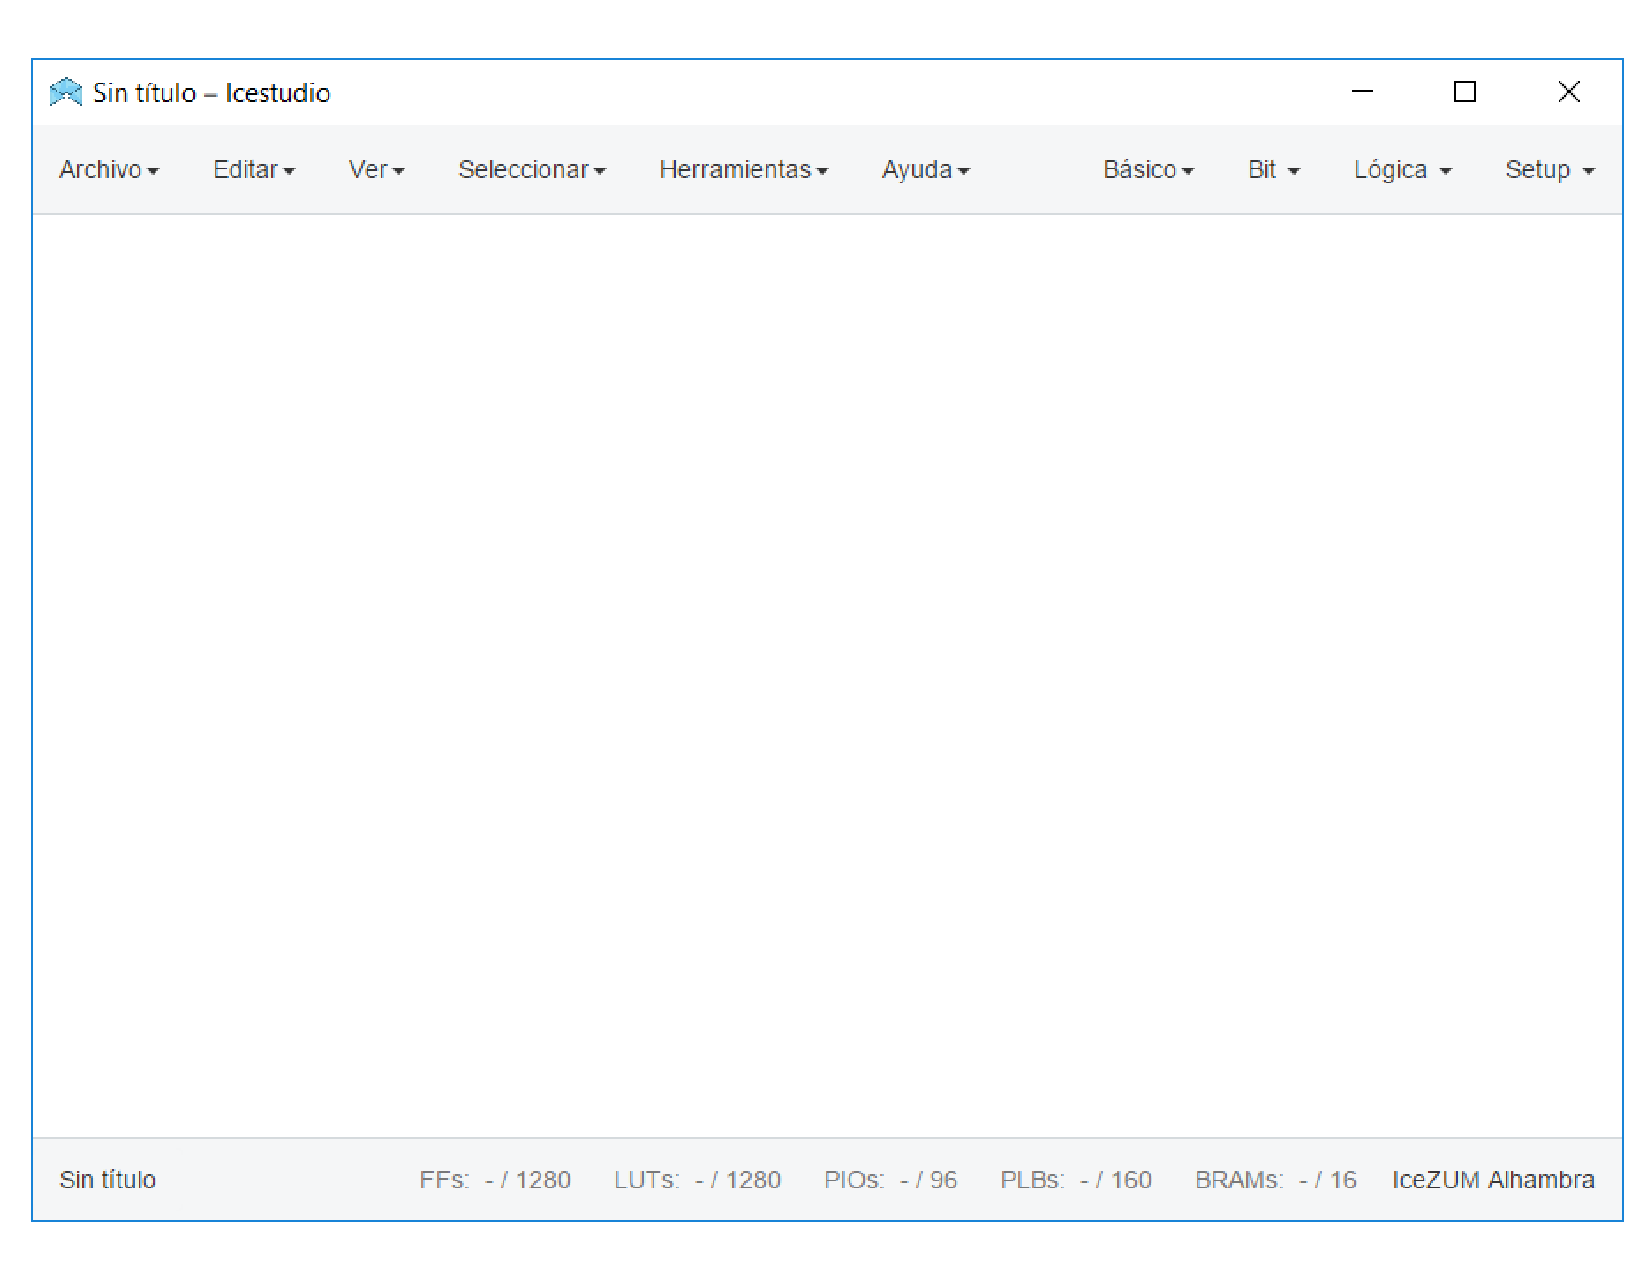
\includegraphics[trim = 0mm 20mm 0mm 0mm, clip,scale=0.4]{imagenes/EstadoArte/Main_IceStudio.pdf}
	\caption{Main Window IceStudio.}
	\label{fig:Main_IceStudio}
\end{figure}

The fact that IceStudio is a graphic editor can make believe that the abstraction level could be higher that desired, but the truth is that this a configurable level. The final user who decides which abstraction level will be working with, making necessary for this a large modules library as we will se ahead. In order to explain the IceStudio power, a practical case will be shown.\newline

The module represented in figure \ref{fig:Write_i2c_module} is a normal writing of i2c, in which the slave direction is parameterized and also the direction that wants to be read on (will be explained in detail ahead). \newline

\begin{figure}[H]
	\center
	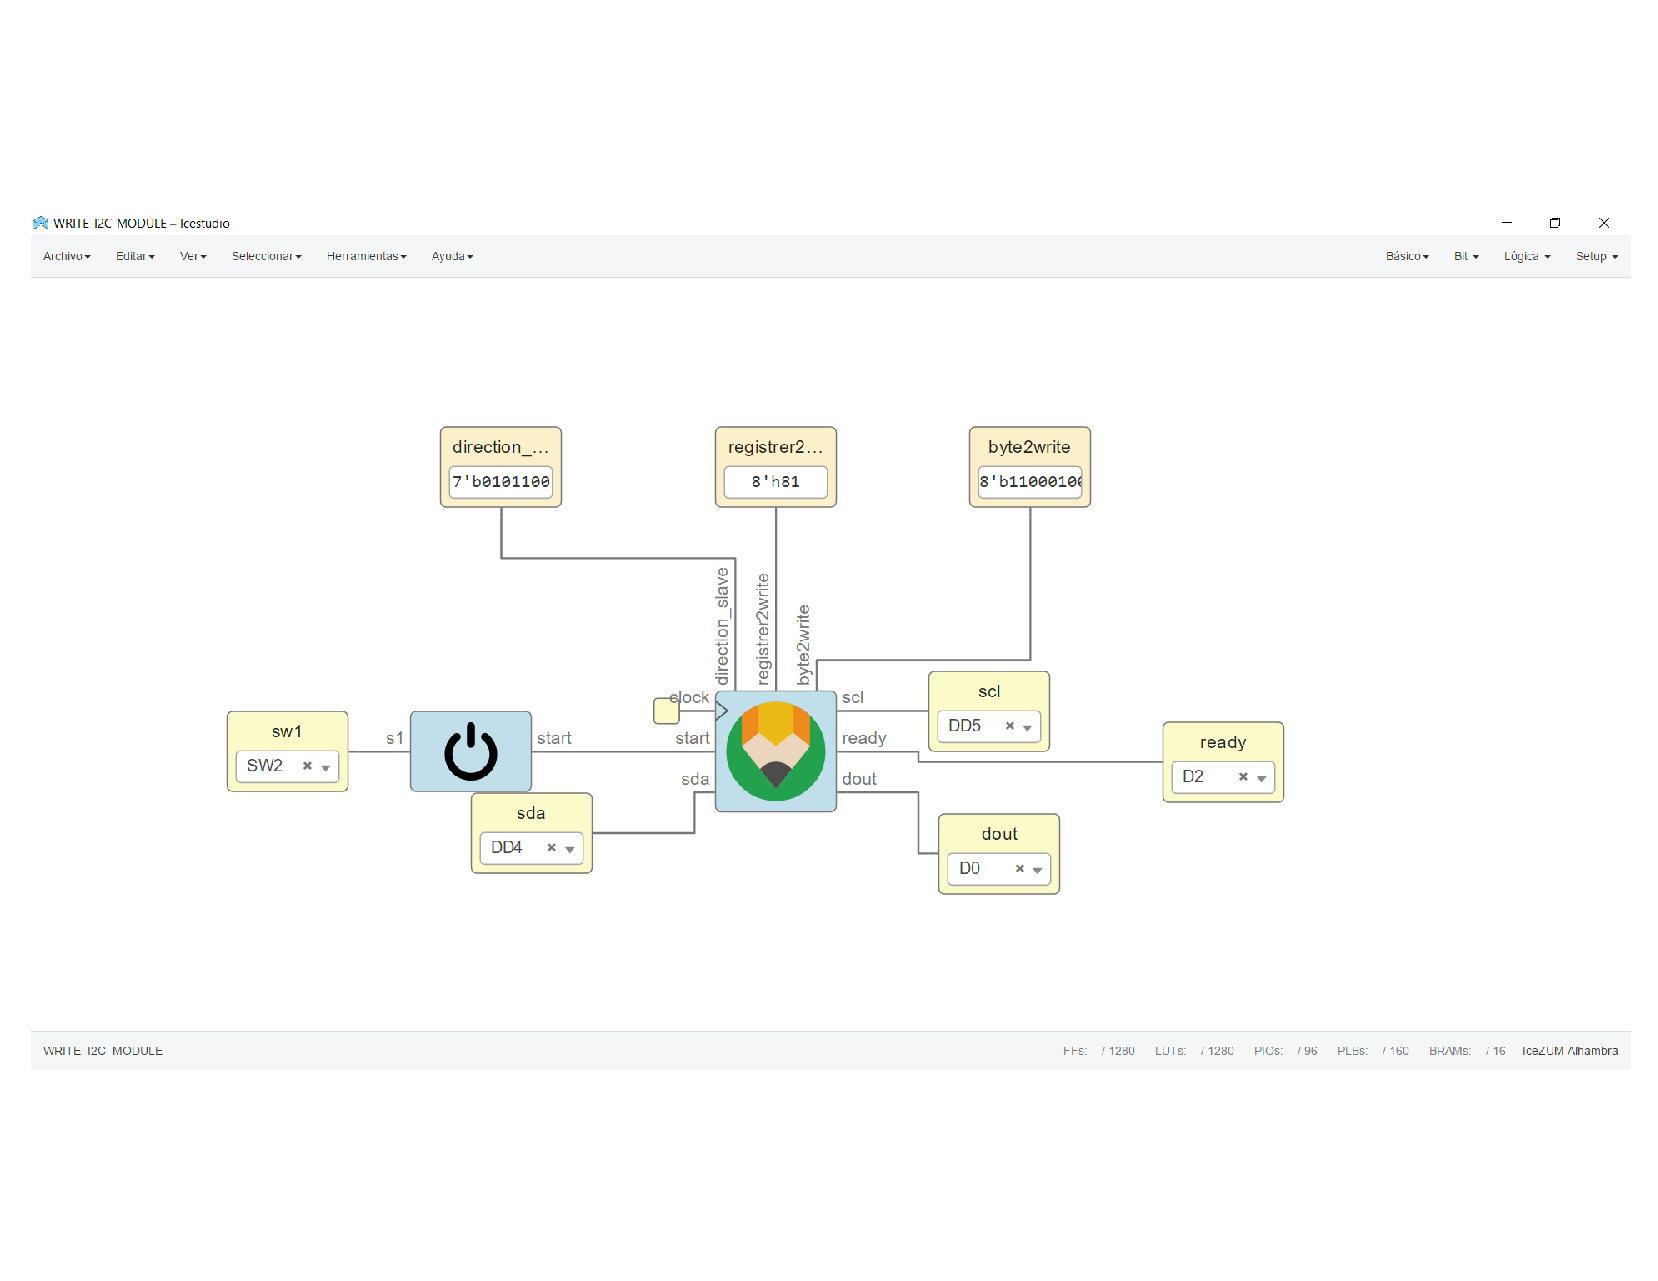
\includegraphics[trim = 0mm 25mm 0mm 0mm, clip,scale=0.4]{imagenes/EstadoArte/Write_i2c_module.pdf}
	\caption{High-Level I2C writing}
	\label{fig:Write_i2c_module}
\end{figure}

Thus, if someone who is not familiarized with this type of code and whose objective is not to understand it but wants to make use of it, it should not lower a lot of level.
However, there is a possibility that it is necessary to change some values such as clock frequency, i2c operation mode, etc. To do this we can lower the level and enter the module being worked with, in this case, by double clicking, as shown in figure \ref{fig:Write_i2c_module2}. 

\begin{figure}[H]
	\center
	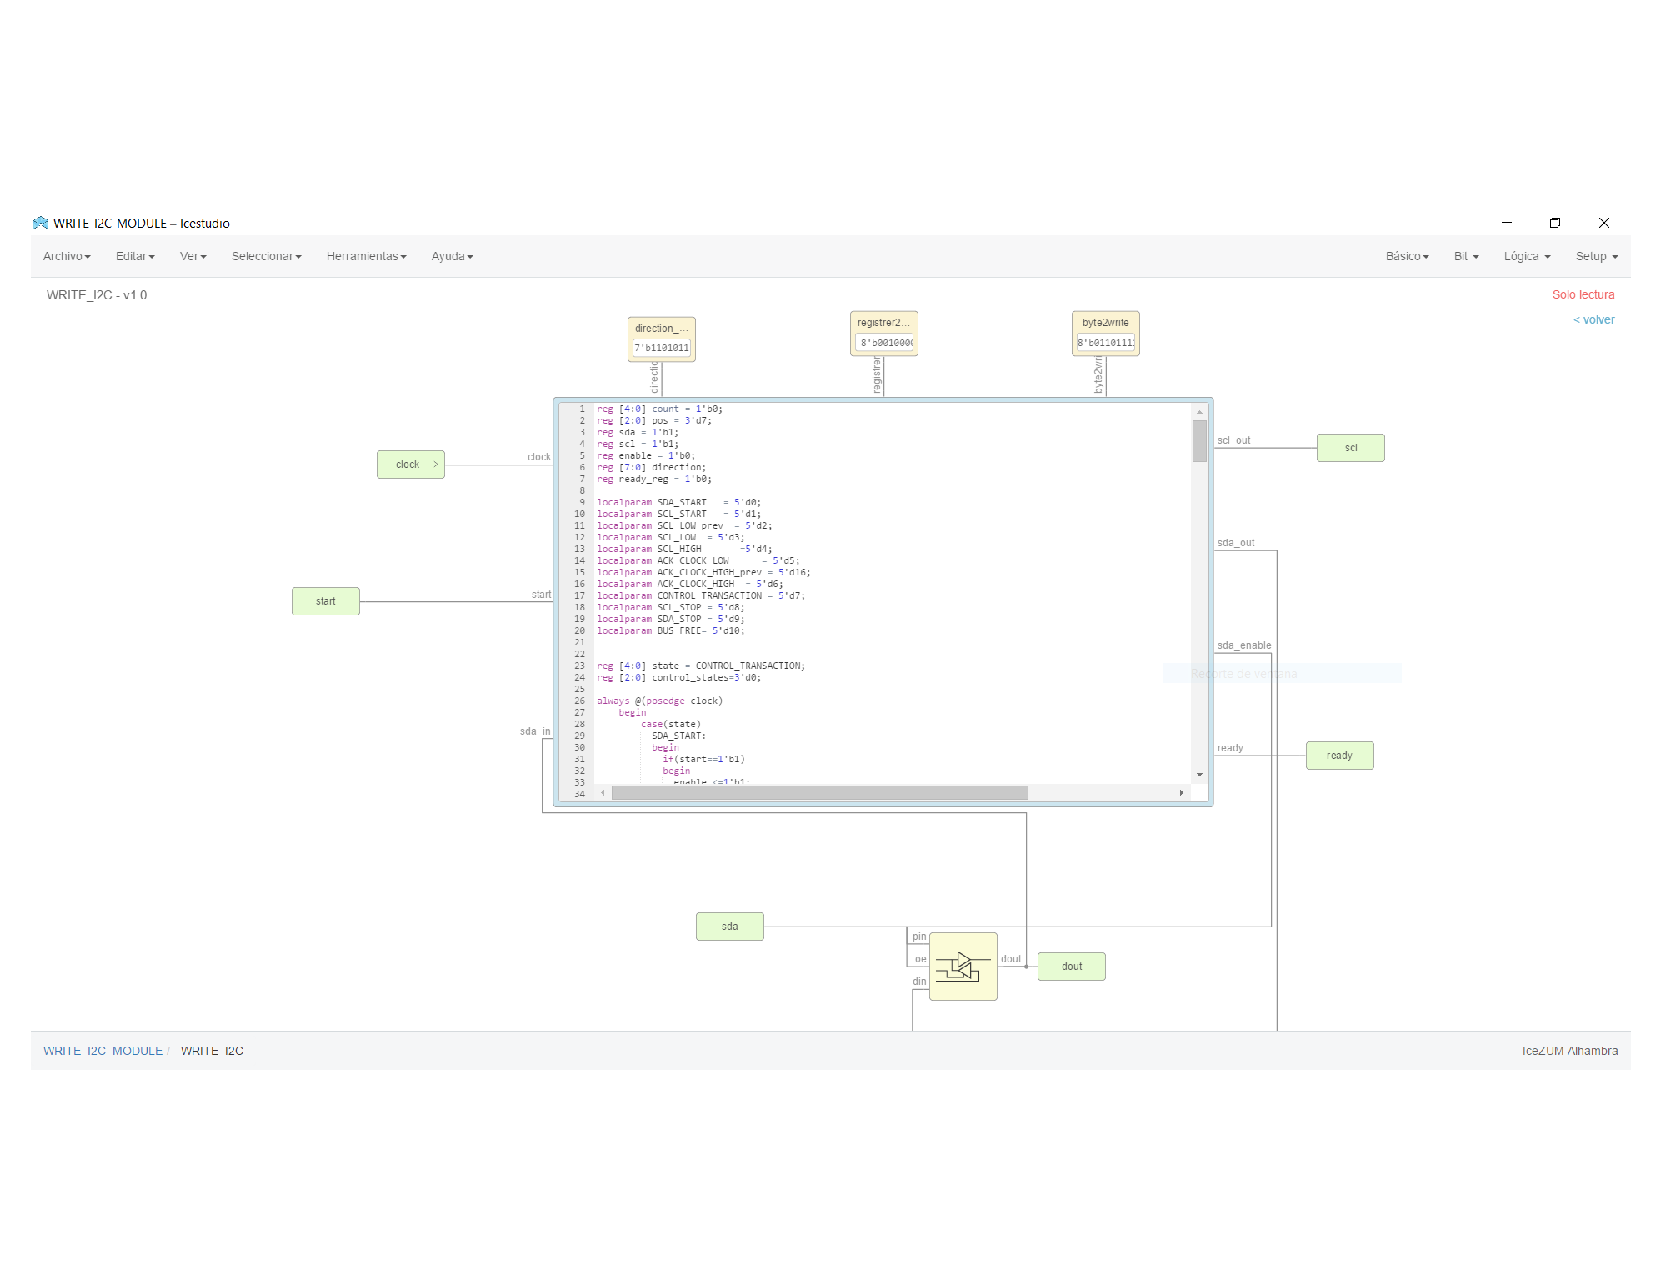
\includegraphics[trim = 0mm 1.5cm 0mm 0mm, clip,scale=0.4]{imagenes/EstadoArte/Write_i2c_module2.pdf}
	\caption{Low-Level I2C writing}
	\label{fig:Write_i2c_module2}
\end{figure}

The it could be said that a level of abstraction has been lowered, being now able to enter in more specific hardware details if necessary. \newline

In the previous practical case, one of the advantages of IceStudio has been seen. Modularity allows to configure the abstraction level. For this, we need a module’s library, some of which will be developed throughout this work, some other modules are being developed, and can be found at \cite{GoogleGroups}.

%%%%%%%%%%%%%%%%%%%%%%%%%%%%%%%%%%%%%%%%%%%%%%%%%
\section{Microcontroller-FPGA coexistence}\label{sec:coexistencia}
\subsection{Microcontroller-FPGA differences}
At first it may seem that a processor and FPGA are similar devices because both can perform certain pre-configured tasks. The truth is that digging deeper we can find more differences than similarities. Both are able to implement a transfer function, but the way they do it is different for each of them.\newline

This, we could see FPGA and microcontrollers in a black box in which we have some inputs and several outputs as shown in figure \ref{fig:funcionalidad_FPGA_micro}.\newline


\begin{figure}[H]
	\center
	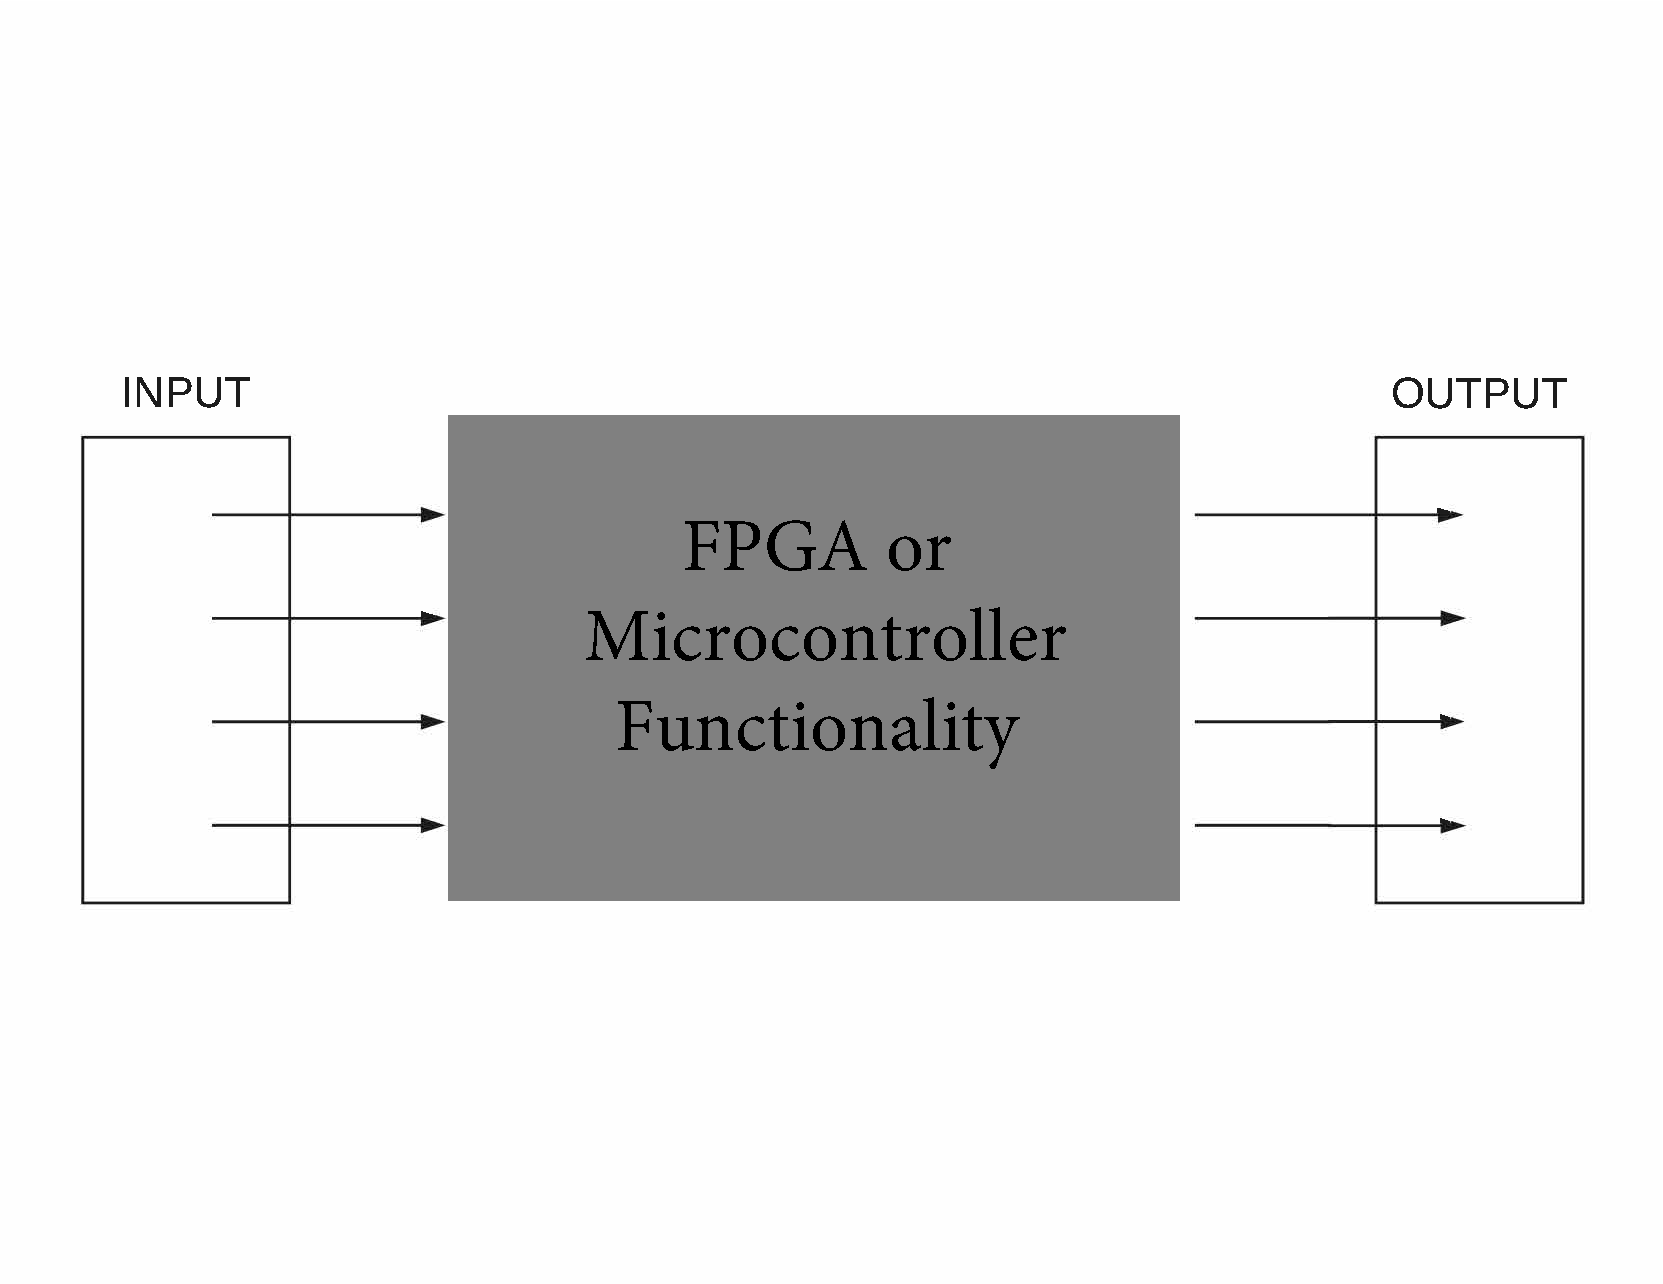
\includegraphics[trim = 0mm 30mm 0mm 30mm, clip,scale=0.4]{imagenes/EstadoArte/funcionalidad_FPGA_micro.pdf}
	\caption{Funcionalidad FPGA y Micro-controlador.}
	\label{fig:funcionalidad_FPGA_micro}
\end{figure}

To summarize how they implement this transfer function differently, the way to work with a processor will be briefly explained. \newline
A processor contains a series of instructions that perform operations on a set of bits (add, increase, read and write in memory). Depending on the processor type and its architecture we have more or less associated instructions, this being one of the most important aspects that determine its performance. 

\begin{center}
	\begin{figure}[H]
		\center
		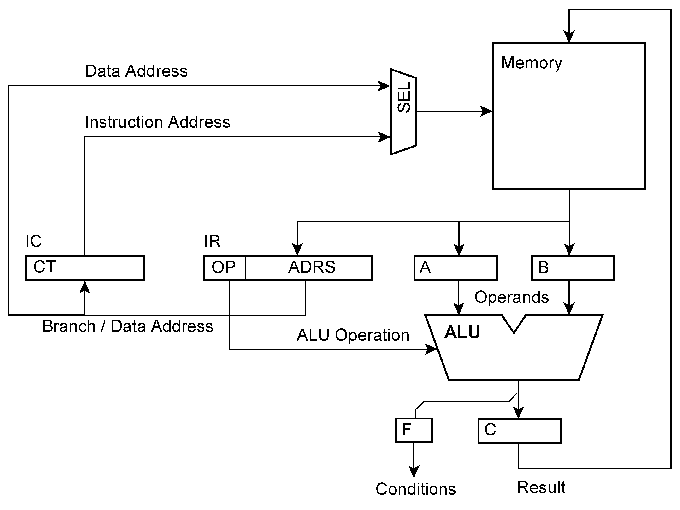
\includegraphics[scale=0.3]{imagenes/EstadoArte/processor.png}
		\caption{Basic architecture in a processor}
		\label{fig:arquitectura_procesador}
	\end{figure} 
\end{center}


It has a series of registers, a memory to store the information and a stack of instructions, which contains the program to be executed in machine code, in addition to a clock.\newline

Its operation mode at a high level; in each clock cycle the processor reads from its instruction stack all necessary values, calls the appropriate instruction and executes a determining calculation.\newline
As discussed in \ref{sec:ArquitecturaFPGA}, when implementing a logic design in an FPGA, a matrix of physical connections is being modified. By modifying that connection matrix, different functionality blocks can be implemented, which means, it could be represented as several transfer functions in a same hardware system.\newline
Figure \ref{fig:puertas_logicas} shows a real example of how the physical connections of logical gates are implemented in an FPGA, and how it allows to have independent modules from each other. Also, notice the problem of the memory in an FPGA, being this the total number of physical logical doors that can be used.
\begin{center}
\begin{figure}[H]
	\center
	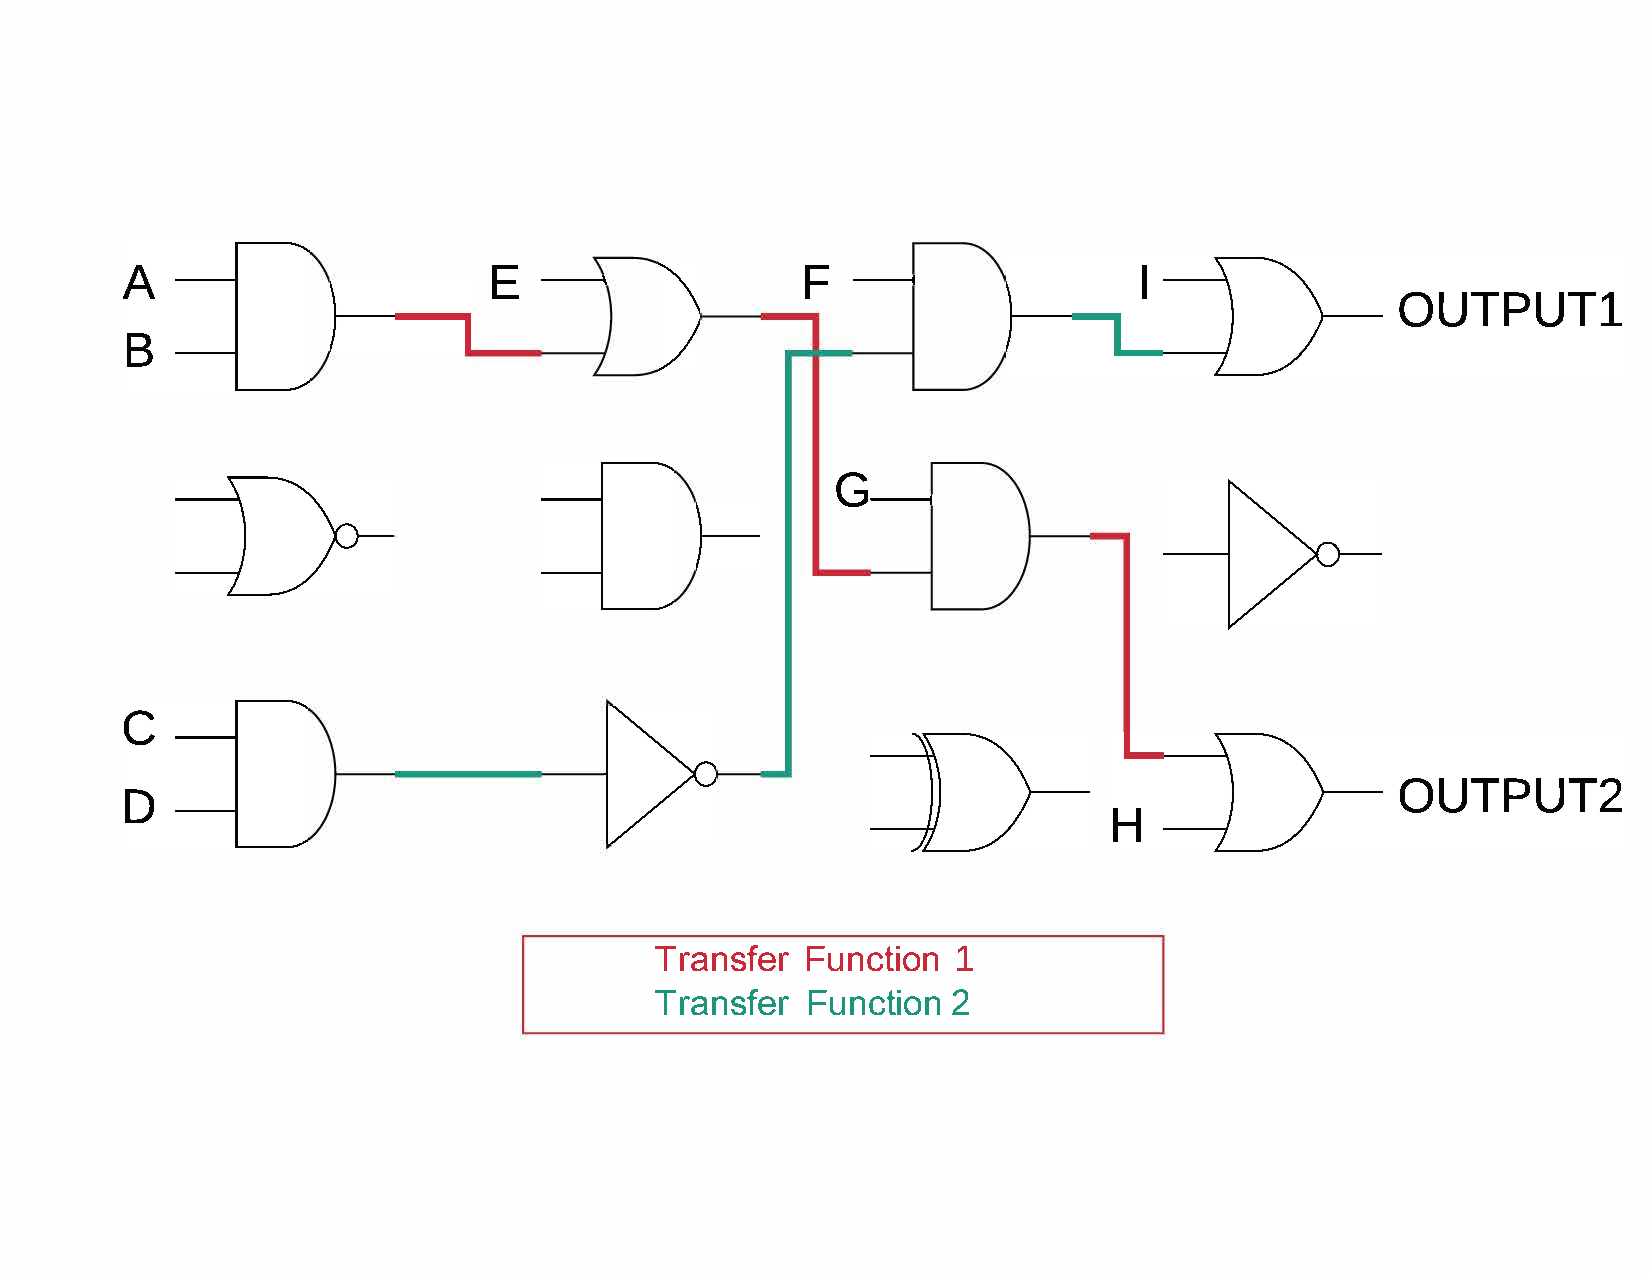
\includegraphics[scale=0.3]{imagenes/EstadoArte/puertas_logicas.pdf}
	\caption{Logic gates in a hardware implementation.}
	\label{fig:puertas_logicas}
\end{figure}
\end{center} 

\subsection{Importance}

The following practical case is proposed:\newline

\textsl{It is required to monitor with accuracy 4 different sensors coming from the outside, in an exact way, all four at the same time and at a specific speed by an external clock, being necessary in addition an actuation of the system (valve opening, closes gates, etc).}\newline

The workflow block diagram in a processor that implements the above, might look like figure \ref{fig:processor_sensor}

\begin{center}
	\begin{figure}[H]
		\center
		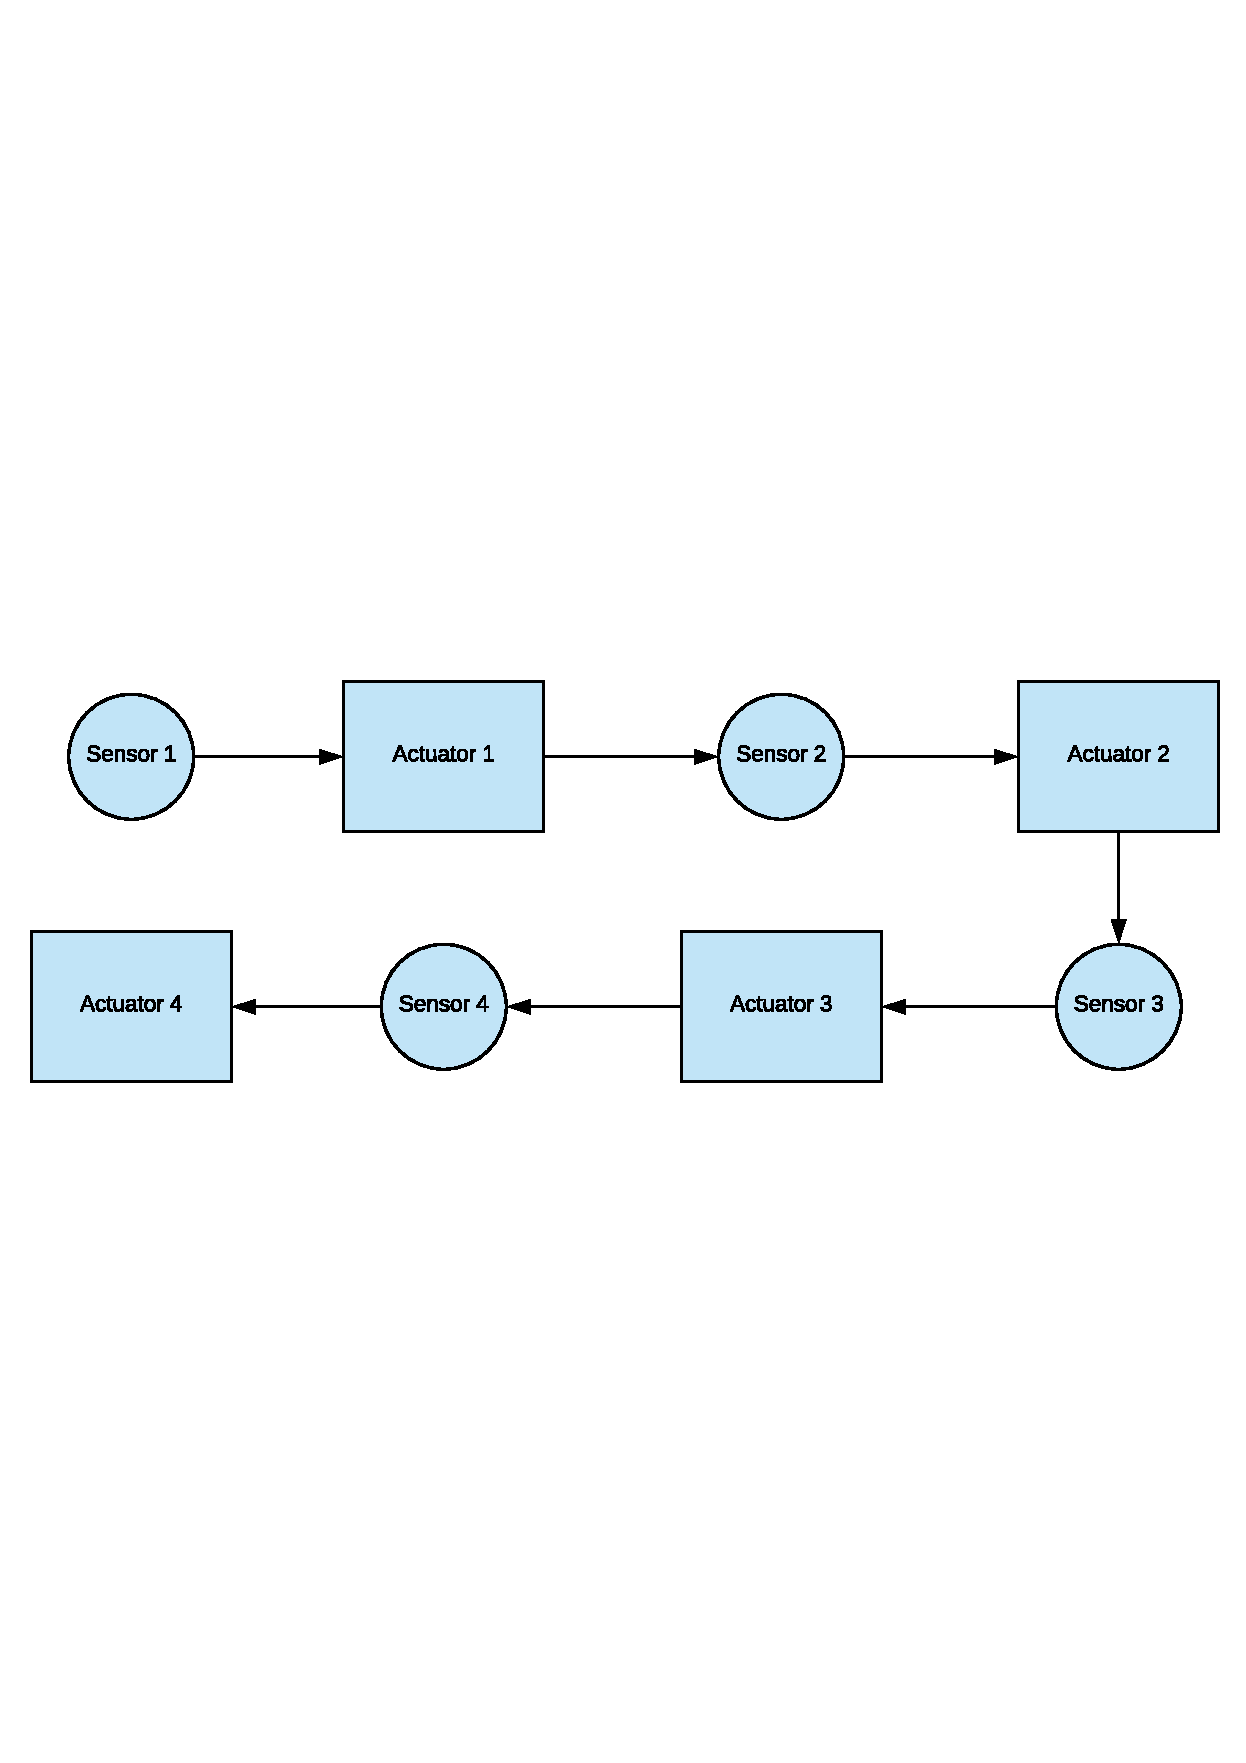
\includegraphics[trim = 0mm 10cm 0mm 10cm, clip,scale=0.5]{imagenes/EstadoArte/processor_sensor.pdf}
		\caption{Flow diagram in a processor.}
		\label{fig:processor_sensor}
	\end{figure}
\end{center} 


Thus, the end user of this system should be able to check in a cyclic way, each sensor and its following performance, thus failing to meet the specifications (the four sensors will not be monitored at the same time).
If the work was done with interruptions, the different external interruptions would be configured or cyclic executives would be used in order to approach those final requirements. However, any of these solutions, they are still an approximation.\newline
In contrast, with the use of an FPGA, the block diagram of the workflow would look like figure \ref{fig:fpga_sensor}.

\begin{center}
	\begin{figure}[H]
		\center
		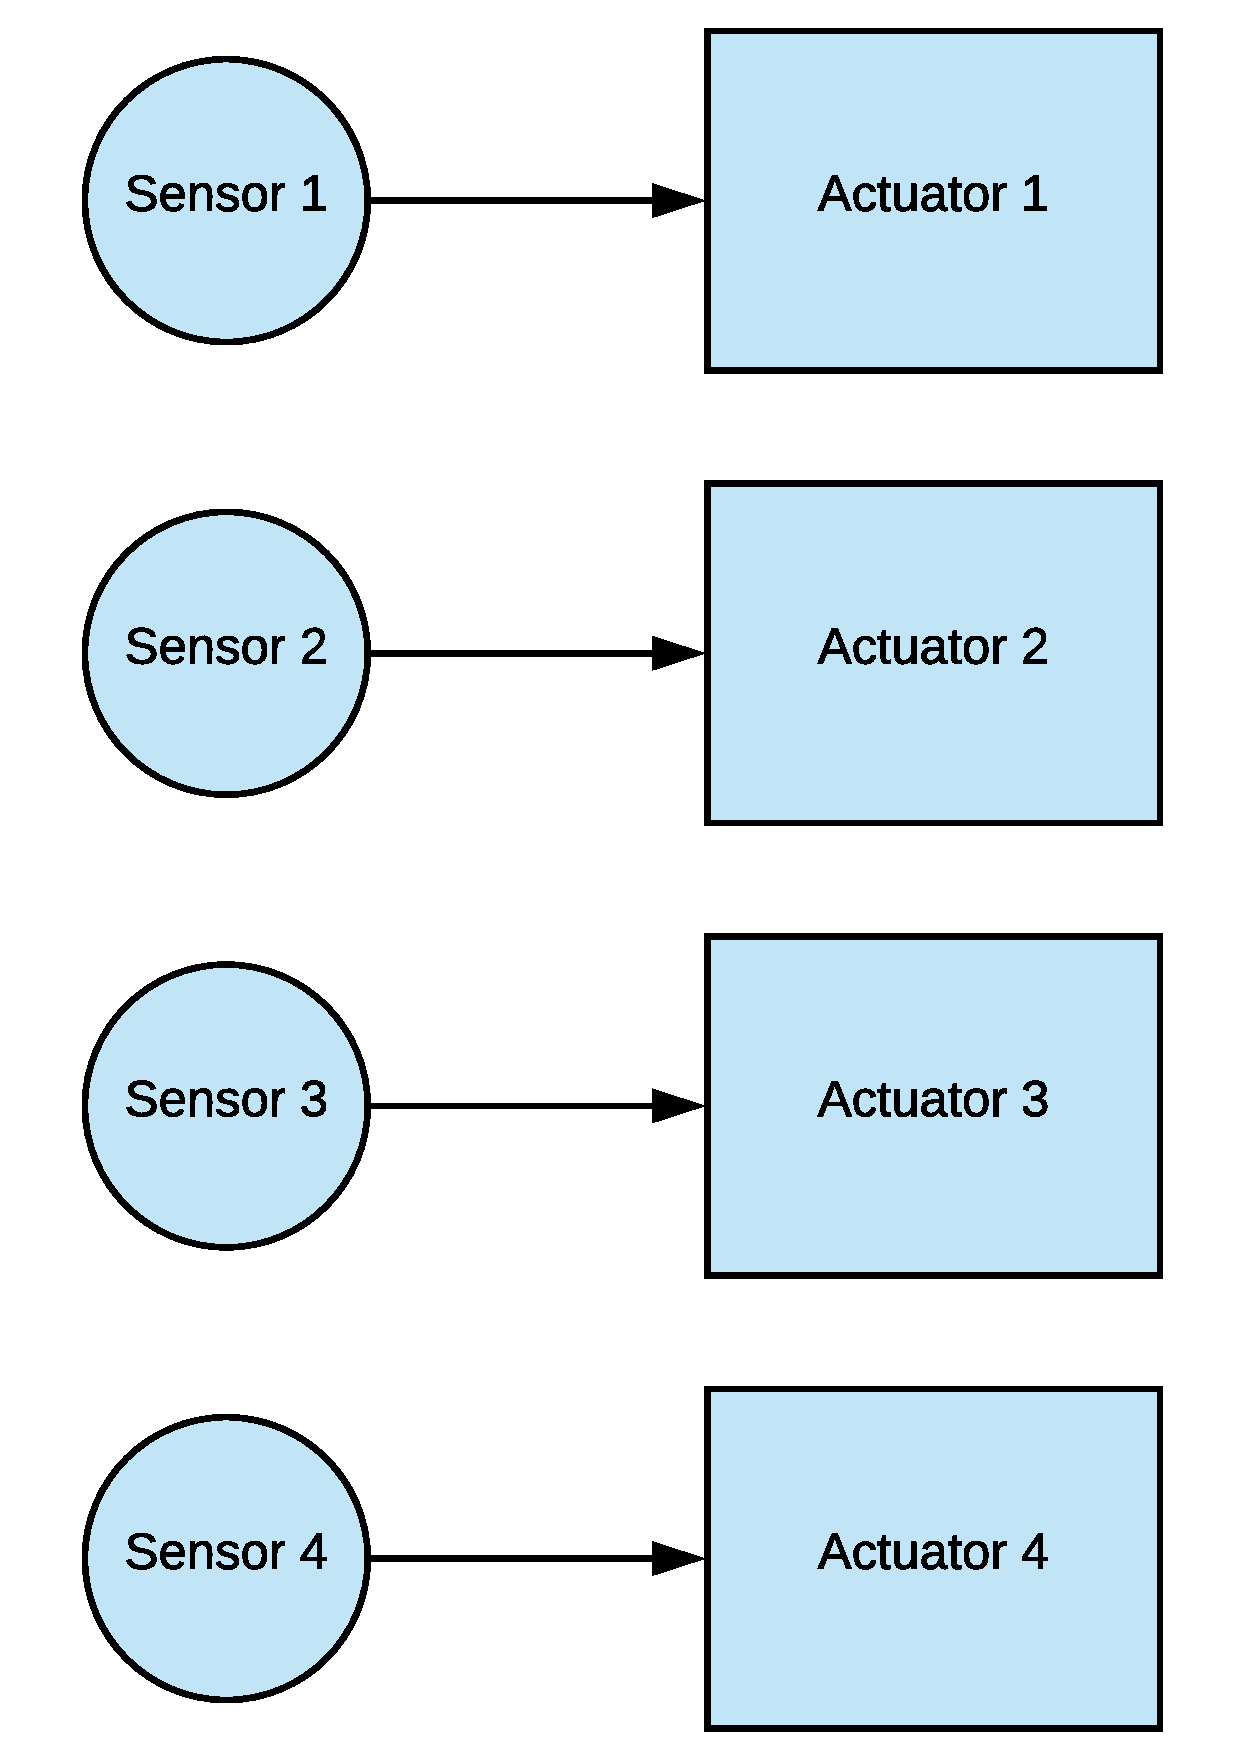
\includegraphics[trim = 0mm 0mm 0mm 0mm, clip,scale=0.3]{imagenes/EstadoArte/fpga_sensor.pdf}
		\caption{Flow diagram in a FPGA.}
		\label{fig:fpga_sensor}
	\end{figure}
\end{center} 


Different transfer functions will be implemented for each one of the blocks to be developed, which can be executed in parallel.
However, it is not always necessary to have parallel execution, and not only may it not be necessary, but it could be harmful. When a system must be sequential, why to use a parallel nature implementation? \newline

It is very common to have systems where it is convenient to be able to implement both types of operation, for that reason an FPGA/Microcontroller coexistence could be enough to adapt to the requirements. \newline

In figure \ref{fig:bipedo} a real example of a bipedal system can be seen, which would be more detailed explained in the following chapters.

\begin{center}
	\begin{figure}[H]
		\center
		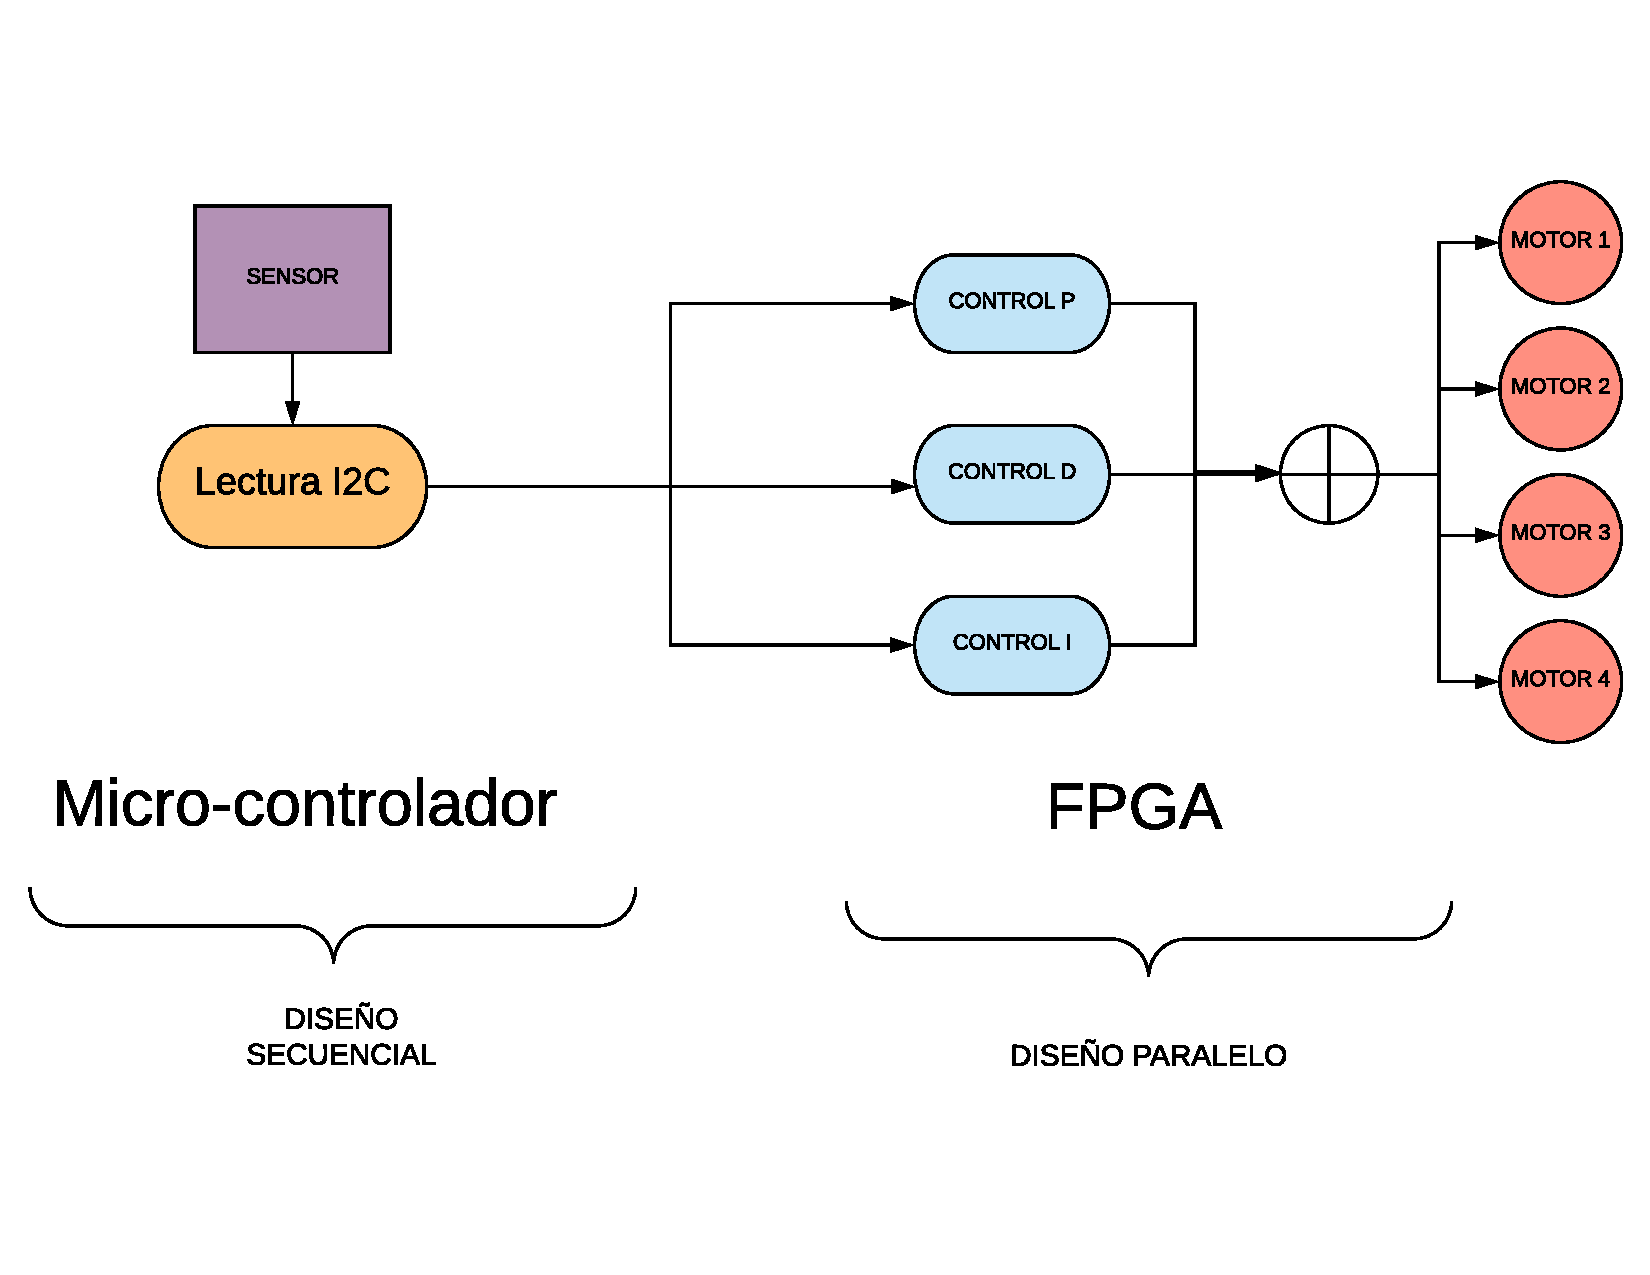
\includegraphics[scale=0.4]{imagenes/EstadoArte/bipedo.pdf}
		\caption{Bipedal System coexistence between microcontroller and FPGA.}
		\label{fig:bipedo}
	\end{figure}
\end{center}
%%%%%%%%%%%%%%%%%%%%%%%%%%%%%%%%%%%%%%%%%%%%%%%%%
\newpage
\section{Inertial Measurement Unit}\label{sec:IMU}
The central component of the proposed system is defined as IMU or inertial measurement unit. It is composed of a series of sensors which will be used to know exactly many on-board location system aspects such as speed, orientation, gravitational forces, etc. \newline
This information can be used for control or simple knowledge of the system at a specific time. \newline

In the case of the present project, it will be used to obtain the navigation angles or Tait-Brain angles, in which the orientation is presented with three orthogonal rotations around the X, Y and Z axis. An example of this type of representation can be found in Figure \ref{fig:orientacion}.\newline


\begin{figure}[H]
	\center
	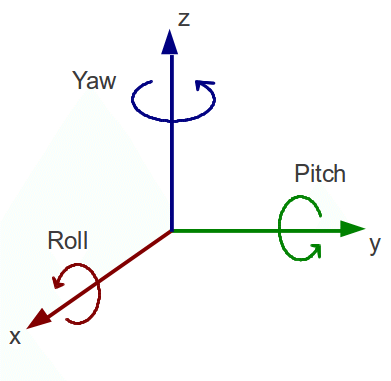
\includegraphics[scale=0.5]{imagenes/Balancing_robot/orientacion}
	\caption{Tait-Brain angles.}
	\label{fig:orientacion}
\end{figure}


An IMU is defined by its number of degrees of freedom (DOF) which would depend on the number of sensors on board (accelerometer, gyroscope) and the number of axis on which are applied. Thus, an IMU with six DOF (for example a 3-axis accelerometer and a 3-axis gyroscope) would be said to be 6DOF. \newline

Figures \ref{fig:IMU12}, \ref{fig:IMU2}, \ref{fig:IMU2} present some IMUs examples.

\begin{figure}[H]
	\center
	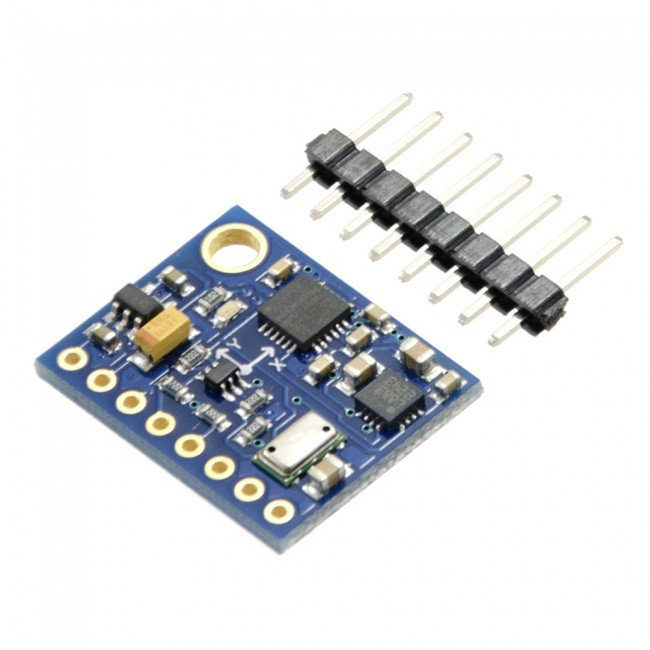
\includegraphics[scale=0.2]{imagenes/Balancing_robot/IMU1}
	\caption{IMU.}
	\label{fig:IMU12}
\end{figure}

\begin{figure}[H]
	\center
	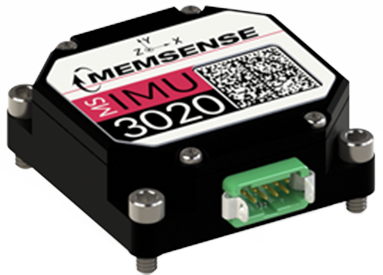
\includegraphics[scale=0.2]{imagenes/Balancing_robot/IMU2}
	\caption{IMU.}
	\label{fig:IMU2}
\end{figure}

\begin{figure}[H]
	\center
	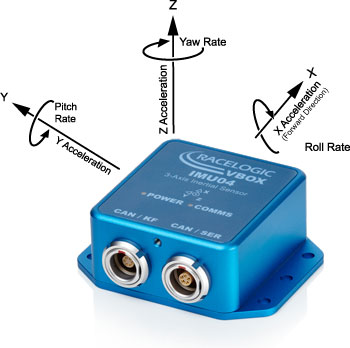
\includegraphics[scale=0.25]{imagenes/Balancing_robot/IMU3}
	\caption{IMU.}
	\label{fig:IMU3}
\end{figure}

Another important feature and one on which will largely depend the price of the product, is the range of the on-board sensors and the availability in the digital analogous converters system, which are in charge to convert the value of the sensor to a binary value that can be used for further analysis. \newline
Following there are some of the most important aspects that can be found in an Inertial Measurement Unit and those that would be very useful throughout the present project.

\subsubsection{Accelerometer}
An accelerometer, as its name suggests, is a device that allows measuring the acceleration to which a body is subjected. It is a fundamental component in the inertial measurement units because it can detect, for example, free fall conditions, although the main use is to determine the sensor’s orientation.\newline

Normally accelerometer have 3 axis, which means, they are capable to independently measure the acceleration in X, Y and Z axis, which allows to know the magnitude and direction of the acceleration vector on each one of the axis. \newline

The important case in this project is to be able to determine the sensor orientation. For that, trigonometry must be applied. Supposing a 2D system according to Figure \ref{fig:acelerometro1}.

\begin{figure}[H]
	\center
	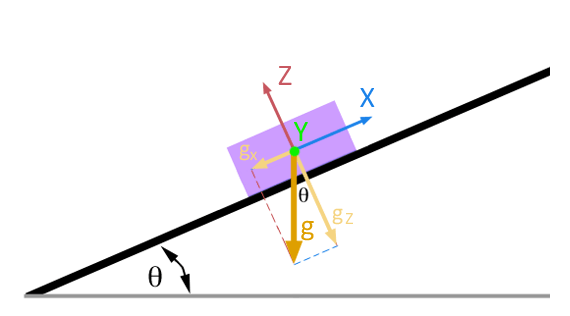
\includegraphics[scale=0.4]{imagenes/Balancing_robot/acelerometro1}
	\caption{Trigonometry in accelerometer system 2D.}
	\label{fig:acelerometro1}
\end{figure}

\begin{equation}
\theta = atan\frac{A_{x}}{A_{z}}
\end{equation}

If it is applied in a 3D representation as shown on Figure \ref{fig:acelerometro2}

\begin{figure}[H]
	\center
	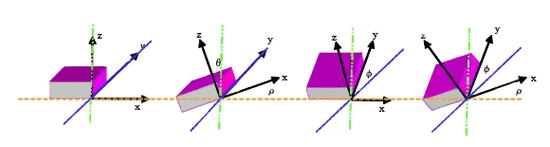
\includegraphics[scale=0.6]{imagenes/Balancing_robot/acelerometro2}
	\caption{Trigonometry in accelerometer system 3D.}
	\label{fig:acelerometro2}
\end{figure}

\begin{equation}
\theta_{x} = atan\frac{A_{x}}{\sqrt{A_{y^2}+A_{z^2}}}
\end{equation}

\begin{equation}
\theta_{y} = atan\frac{A_{y}}{\sqrt{A_{x^2}+A_{z^2}}}
\end{equation}

\begin{equation}
\theta_{z} = atan\frac{A_{z}}{\sqrt{A_{x^2}+A_{y^2}}}
\end{equation}

\subsubsection{Gyroscope}
A Gyroscope is a device that allows to measure the rotation angle of a certain device. \newline

In a gyroscope, relative angles are always measured to an arbitrary reference (unlike accelerometers). Gyroscope used in this project is called a Coriolis Vibratory Gyroscope. \newline

As in the accelerometer in the previous section, gyroscopes usually employ three axes, that is, they are able to independently register the rotation in the X, Y and Z axis, so the module and direction of the rotation vector are obtained.\newline

It is important to keep in mind that this kind of Gyroscopes based in Coriolis effect are not able to detect the rotated angle, but the angular speed, an important aspect to its depuration. \newline

Reminding the angular speed concept (\ref{equation:velangular}):

\begin{equation} \label{equation:velangular}
\omega = \frac{\delta \omega}{\delta t}
\end{equation}

In order to obtain the angle, it is necessary to perform the integration with respect to time (ecquation \ref{equation:integracion}):

\begin{equation}\label{equation:integracion}
\theta_{gyro} = \omega_{gyro}*\Delta t
\end{equation}

Accelerometers are devices that are often very sensitive to vibrations, so for its correct processing must take into account that it will present a lot of high frequency noise. A filtering at a certain frequency will solve part of this problem.\newline

Having to make an integration with respect to time brings with it some problems which would be seen in the next section.

\subsubsection{Drift Problem}

A huge part of the Inertial Measurement Units on the market are at least composed with accelerometers and gyroscopes, the reason for this combination is that one complements the limitations of the other and vice versa. \newline

The drift in an electronic sensor is a variation over time of the output of the meter (with respect to the real measurement) although the variable may be constant, is in a way cause by extent changes in the temperature or by the accumulation of errors. \newline

In both accelerometer and gyroscope, we find drift associated errors: 
\begin{itemize}
	\item Accelerometers do not have medium or long-term drift; however, they are influenced by the movements of the sensor and the noise, reason why they are not reliable to medium or short term.
	\item As for gyroscopes, they work very well in sudden and short movements but when making an integration with respect to time the drift problem appears in the medium or long term.
\end{itemize} 

After analyzing both accelerometers and gyroscopes problems, it seems reasonable to combine both measurements to obtain more precise orientations.

\subsubsection{Possible solutions}

To solve some of the above problems, it can be very useful to apply some of the following proposed solutions: 

\begin{itemize}
	\item Combine and filter the signals by using a complementary filter. It is the most used nowadays due to its not very high complexity. Its simplest expression is represented in equation \ref{equation:complementary_filter}.
	\begin{equation} \label{equation:complementary_filter}
	\theta = A * (\theta_{prev}+\theta_{gyro}) + B * \theta_{accel}
	\end{equation}
	\item Combine and filter the signals using a Kalman filter, which evaluates the future value of the measurement. However, it uses complex calculations. 
	\item Some inertial measurement units internally incorporate DMPs processors (Digital Motion Processor) which execute complex algorithms avoiding having to perform filters and freeing the processing system.
\end{itemize}

One explained the basic features of commercial IMUs, in section \ref{sec:MPU6050} will be developed the IMU chosen for this system and its own features.

\section{Educational Robotics – Motivations}

Robotics\cite{6826237} can be considered as one of the technological areas with more boom nowadays and based on the study of robots, which are systems composed of mechanisms that allow to make movements and perform specific tasks, programmable and intelligent. \newline

Depending on the application, therefore, robotics can be extended and generate benefits not only in the industry but also in classrooms, enabling the appearance of new learning systems.\newline

In addition, in a world whose future is aimed at the use of robots for any activity, the approach from classrooms with these systems, enables the student’s technological development at an early age, making their integration easier into an adult age.\newline

Some robotics educational benefits are:  
\begin{itemize}
	\item Drives initiative and creativity
	\item Larger sociability
	\item Encourages algorithmic and mathematical thinking
	\item Teamwork
	\item Problem resolution
	\item Active learning.
	\item Self-Esteem increase.
\end{itemize}

However, so that the integration in the classroom of educational robotics could be easier, the systems must fulfill some characteristics:

\begin{itemize}
	\item High technological integration level not recommended
	\item Robots must be sociable and fun
	\item Programming environments should not be complex, and even its functionality is kind of limited, it has to draw the attention of the student and make them feel comfortable.
	\item It is important that the robot has a series of sensors and actuators, inputs and outputs so that results must be visuals.
\end{itemize}

After analyzing the advantages of digital electronics, it is convenient to be able to bring these two knowledge fields closer together; educational digital-robotics electronics.\newline

If digital electronics and the world of robots are called to be part of our lives in the near future, the need of an approach to these two concepts at an early age is basic for a correct technological improvement. \newline

IceStudio was born with this idea, making digital electronics to be friendly so that the little aged students can use it, and so, meets the requirements before explained.

\section{Sensors, actuators and control system}

Before starting the development of the project, it is important to be clear about the concepts of sensors, actuators and elements of the control system, which are part of any mobile robotic platform.\newline

Any control installation, being robotic or imnotic, is composed by three fundamental components.
\begin{itemize}
	\item Sensors
	\item Actuators
	\item Control systems
\end{itemize}

Sensors are devices that collect information from the world around us and transform it into electrical signals that can be input to a control system. \newline

Thus, the control system receives information from the environment on which we want to perform some kind of action through the sensors, which is the transfer function of the system. From some known type inputs, outputs are generated, usually, dependent on the inputs.\newline

These outputs are called actuators, which are devices that, following the parameters given by the control system, perform actions that affect the environment. \newline

\begin{ejemplo}
A sensor indicates to the control system the luminous intensity of a room. The control system recognized that the luminous level is not adequate for reading and activates an actuator, in this case, a light to balance that level.
\end{ejemplo}

When choosing a specific sensor, it is important to know its operation module, in order to configure or maintain incorporated systems. There are different type of sensors according to:

\begin{itemize}
	\item Ouput: \begin{itemize}
		\item Analogic
		\item Binary
		\item Digitals
	\end{itemize} 
	
	\item Internal structure: \begin{itemize}
		\item Passive
		\item Active
	\end{itemize}
	
	\item Kind of parameter able to detect.
\end{itemize}
 

Another possible classification is that of the application scope, that is, where and what for these sensors are used. \newline
Between the most important technical features from a sensor and making an introduction to the possible vocabulary that will be used, there are:

\begin{itemize}
	\item Measurement range: Domain to the measured magnitude to which the sensor can be applied.
	\item Precision: Expected maximum measurement error.
	\item Offset or zero deviation: Value of the output variable when the input variable is zero.
	\item Sensor sensitivity: Assuming it is input to output and the variation of the input magnitude.
	\item Resolution: Minimum variation of the input magnitude that can be detected at the output.
	\item Drifts: Are other magnitudes, apart from the measure as input magnitude, that influence the output variable.
\end{itemize}

In general, the output signal from these sensors is not suitable for direct reading and sometimes not for processing, which is why conditioning circuits are used Figures \ref{fig:camara_CMOS}, \ref{fig:IMU} and \ref{fig:potentiometer} show some sensors examples.

\begin{center}
	\begin{figure}[H]
		\center
		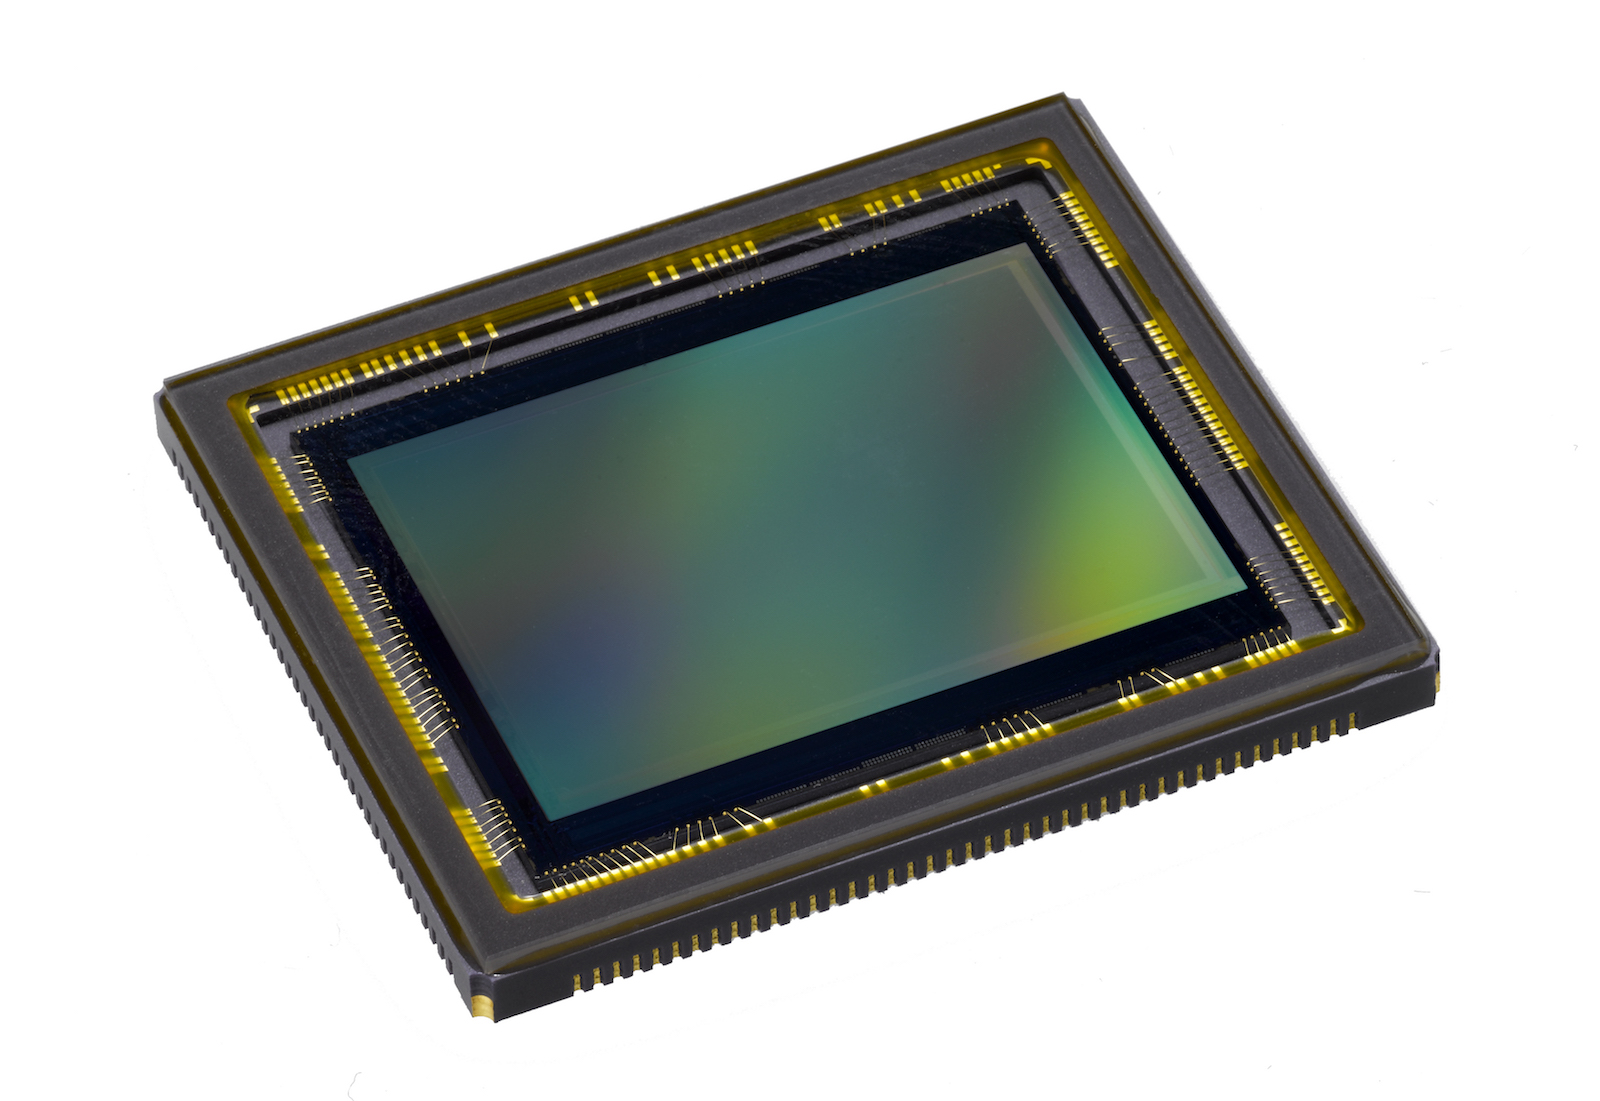
\includegraphics[scale=0.1]{imagenes/EstadoArte/sensor_imagen_CMOS.jpg}
		\caption{Sensor CMOS to image adquisition.}
		\label{fig:camara_CMOS}
	\end{figure}
\end{center}

\begin{center}
	\begin{figure}[H]
		\center
		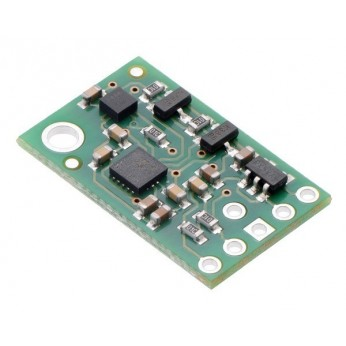
\includegraphics[scale=0.4]{imagenes/EstadoArte/IMU.jpg}
		\caption{IMU.}
		\label{fig:IMU}
	\end{figure}
\end{center}

\begin{center}
	\begin{figure}[H]
		\center
		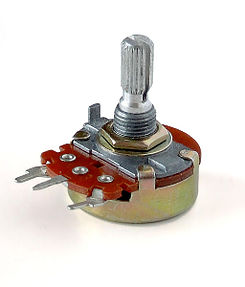
\includegraphics[scale=0.4]{imagenes/EstadoArte/potentiometer.jpg}
		\caption{Potenciometter.}
		\label{fig:potentiometer}
	\end{figure}
\end{center}

Actuators are devices that allow the control system to "act" on the “real world” to perform desired actions. One of the best-known actuators are motors, which will be very used throughout this application.  \newline

\begin{center}
	\begin{figure}[H]
		\center
		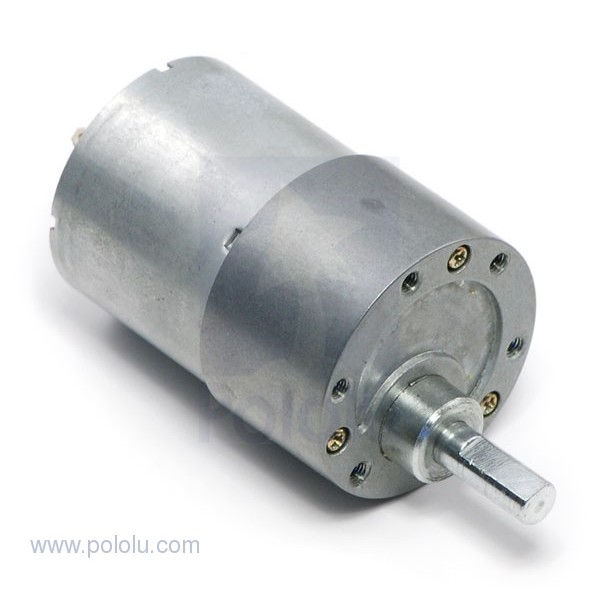
\includegraphics[scale=0.4]{imagenes/EstadoArte/motor.jpg}
		\caption{DC Motor.}
		\label{fig:motor_DC}
	\end{figure}
\end{center}


There are many different types of control systems in relation to the application to be developed, normally a microcontroller is chosen as a control system and the transfer function to be performed is programmed.\newline
In the case of this project, and in order to acquire the advantages of an FPGA and on the other hand the advantages of a microcontroller (seccion \ref{sec:coexistencia}), both Arduino will be used for sequential tasks or the IceZum Alhambra for the tasks that can be parallelized. \newline
\section{Classic PID controller}\label{sec:PID}

Proportional, Integral and Derivative\cite{nemadesign} (Proportional-Integral-Derivative, PID) is the most common and the most used control in the industry and has been universally accepted in the control industry. The popularity of this control is due to its robustness and ease of use, which allows engineers to work in a simple way. \newline

As its name indicates, the algorithm consists in three basic operators: Proportional, Integral and Derivative which are the clue to obtain an optimal response. \newline

The basic idea of a PID controller is to reed a sensor and calculate a proportional response, integral and derivative with the objective of calculating the best output from an actuator. \newline
\newpage
To know very well how a PID controller actuates and to know the meaning of each one of its components, it is necessary to know what a closed loop system is. 

\subsubsection{Closed loop system}
A closed loop control system is s systems in which the action of the control is in function of the output signal. Closed loop systems use feedback from a final result to adjust the control action accordingly. The set point is the value that the system wants to reach. \newline

Now it is digged a little deeper about is what’s the meaning of each of the components by which the PID control is formed.\newline
\subsubsection{Proportional Response}

The proportional component depends only on the difference between the current value and the setpoint. This difference is known as the “Error”. Thus, the proportional gain $K_{p}$ determines the relationship between the output response and the error signal. If the error has a magnitude of 10, a proportional gain of 5 will produce a proportional response of 50. The gain indicates the correction speed of that error, but if it is too fast, the system will oscillate. 
\subsubsection{Integral Response}
The integral component adds the error-in-time component, a small increase in the error until the integral component increases slightly with time. The integral response will increase continuously over time unless the error is zero, so the effect is to bring the steady state error to zero.
\subsubsection{Derivate Response}
The derivative response causes the output to decrease if the process variable increases rapidly. The derived response is proportional to the rate of change of the process variable. Increasing the derivative constant $K_{d}$ will make the control system stronger to changes in the error and will increase the speed of the overall response of the control system. 

A block diagram of the complete system of a PID controller is shown in Figure \ref{fig:PID}.

\begin{center}
	\begin{figure}[H]
		\center
		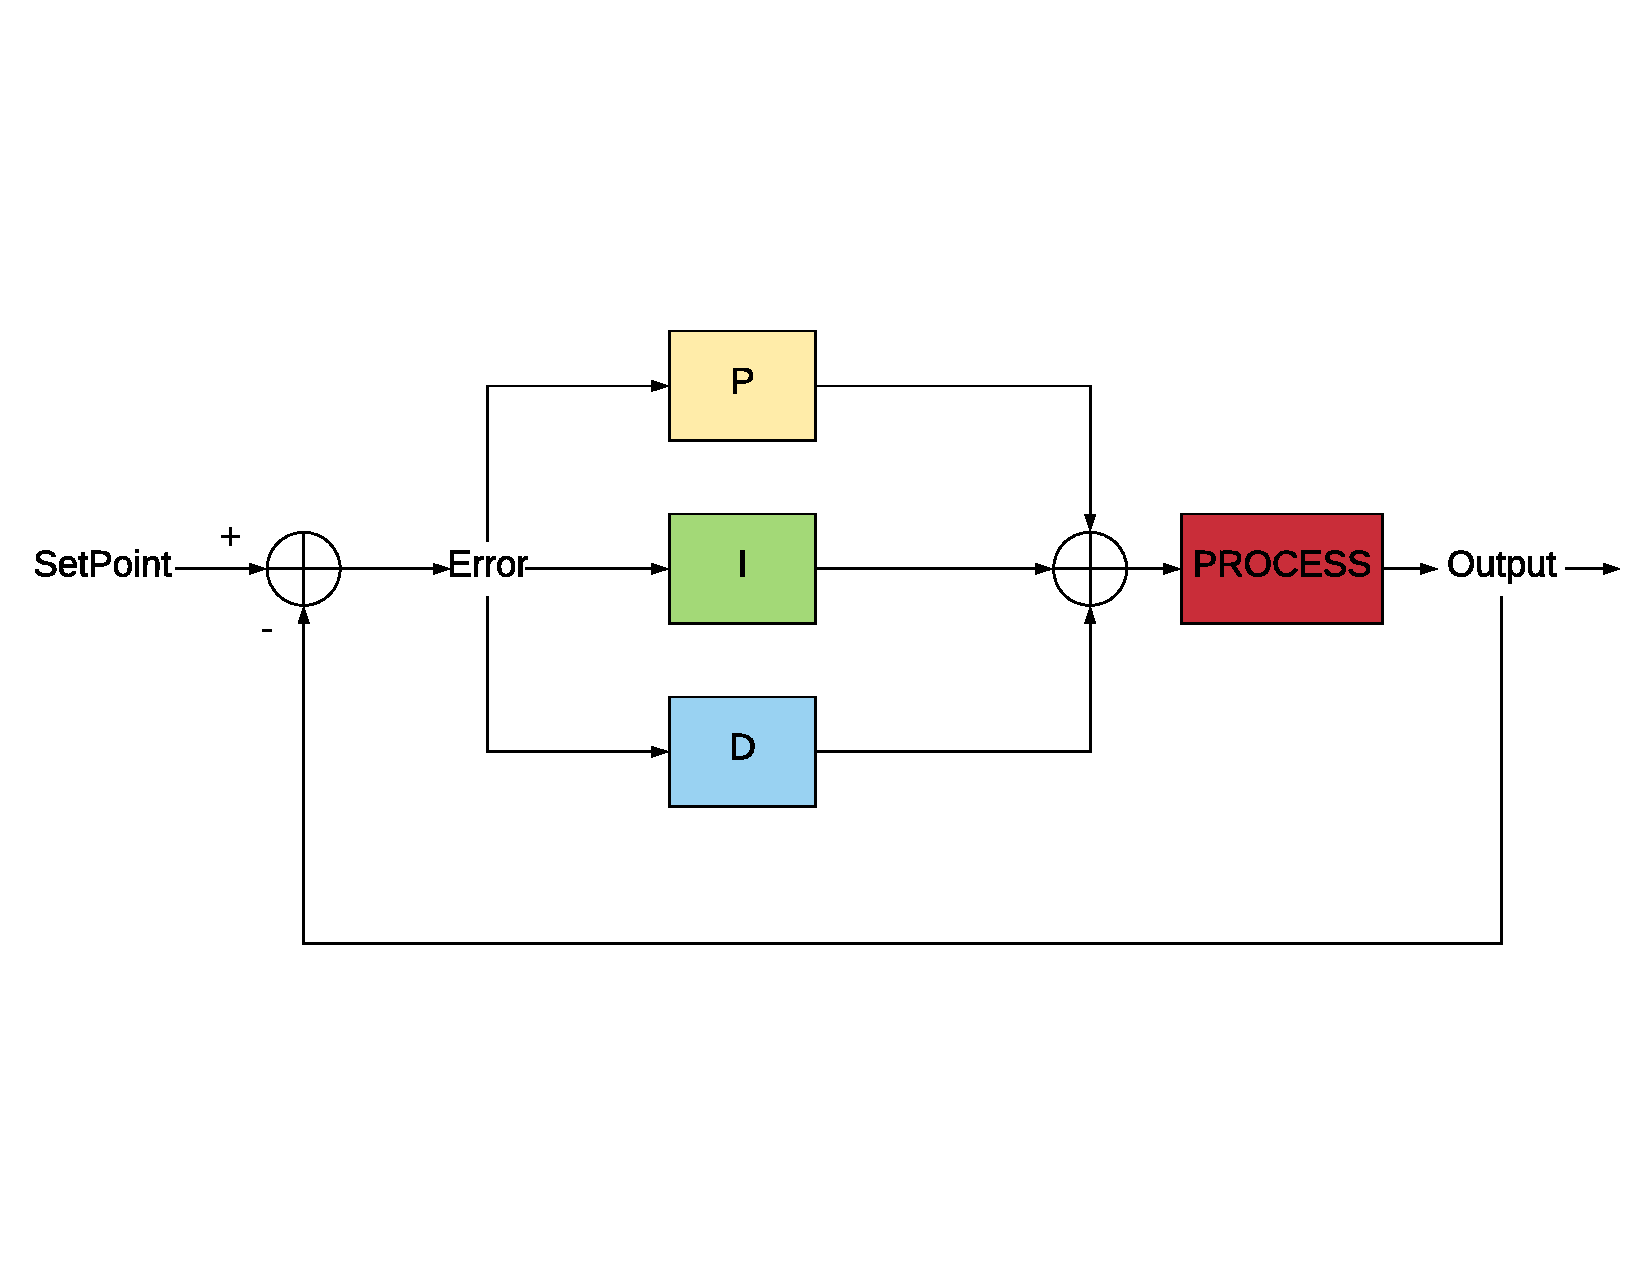
\includegraphics[trim = 0mm 4cm 0mm 4cm,clip, angle=0, scale = 0.4]{imagenes/EstadoArte/PID}
		\caption{Block diagram PID controller.}
		\label{fig:PID}
	\end{figure}
\end{center}

\begin{ejemplo}
A PID is used to control the temperature of a room. The set point is the temperature you want to reach, the plant is the room itself, which can be modeled as a transfer function. A temperature sensor closes the loop, indicating the temperature at each moment, while a valve opens and closes the air duct depending on the values of the PID controller, which will be calculated in relation to the setpoint value and to the value of the current temperature in the room.
\end{ejemplo} 










